\subsection{Results} \label{subsec:results_linear_regression}

\texttt{regression\_analysis/examples/linear\_regression\_analysis.ipynb} is a jupyter notebook which consists of widgets where the statistical performance of different regression methods can be viewed for over a $10^5$ parameter combinations. The data for these experiments is included in the repository. At the end of the jupyter notebook, one can find code that will allow for simulating more parameter combinations if needed. This will overwrite the existing data and also would take a significant time to run. For $10^5$ parameter combinations, it took us about $2$ hours to obtain the data.

\subsubsection{Terminology of symbols and variable names}
Here, we list the names of the variables that are the options in the widgets of the jupyter notebook. The corresponding symbols if applicable are also shown. These symbols relate the variable names to their corresponding mathematical notation used in this report. The general template is the following \\
\\
Symbol: variable name → explanation

The list of widget variables are
\begin{itemize}
    \item $p:$  polynomial order → The order of 2D polynomial used for fitting
    \item $var:$  noise\_var → The variance of the zero mean gaussian noise added to the Franke data
    \item $r:$  ratio → testing ratio. For example, if ratio is 0.1 then the test set comprises of 10 percent of the dataset.
    \item $n:$  num → The number of points taken along each direction of the input vector. If num = 20, then the total number of data points is 20*20 = 400
    \item stat → Displays the chosen statistic
    \begin{itemize}
        \item $MSE_{train}:$ training MSE
        \item $MSE_{test}:$ testing MSE
        \item ${R^2_{train}}:$ training R2 error
        \item ${R^2_{test}}:$ testing R2 error
        \item $bias_{test}:$ bias in test data
        \item $var_{test}:$ variance in test prediction
    \end{itemize}
    \item method → To choose the regression type
    \begin{itemize}
        \item Direct solution and stochastic gradient descent solution available
        \begin{itemize}
            \item OLS
            \item OLS with bootstrap resampling
            \item OLS with crossvalidation resampling
            \item Ridge
            \item Ridge with bootstrap resampling
            \item Ridge with crossvalidation resampling
        \end{itemize}
        \item Direct Solution only(using scikit learn)
        \begin{itemize}
            \item Lasso
            \item Lasso with bootstrap resampling
            \item Lasso with crossvalidation resampling
        \end{itemize}
    \end{itemize}
    \item $n_b:$  n\_boot → number of times bootstrap sampling is performed in the bootstrap method. Changing this for methods that doesn't involve bootstrap sampling will not have any effect
    \item $k_f:$  k\_fold → number of folds in the cross validation method. Changing this for methods that doesn't involve cross validation will not have any effect
    \item $\lambda_r:$  ridge\_lambda → Regularisation parameter for ridge regression
    \item $\lambda_l:$ lasso\_lambda → Regularisation parameter for LASSO regression
    \item learn\_rates → Parameter that controls the descent jump size in gradient descent methods
    \item epoch →
    \item number of batches →
\end{itemize}

\subsubsection{Ordinary Least Squares(OLS)}

Here, we present selected results of linear regression that we find particularly interesting.

Foremost, we look at the $MSE_{train}$ of OLS (see figure \ref{fig:ols1}). We see that the $MSE_{train}$ reduces as the model complexity or polynomial order($p$) increases. In other words, with increasing complexity, our model becomes more flexible. As the input data is an exponential function which can be expressed as a series sum of polynomials, increasing the terms in the fitting polynomial should decrease the $MSE_{train}$. We also see that for large values of test ratio i.e. $r = 0.4$ and low number of data points $n = 100$ which amounts to about $60$ datapoints in the training set, the $MSE_{train}$ is significantly lower for high $p$.

\begin{figure}
\centering
\begin{subfigure}{.5\textwidth}
  \centering
  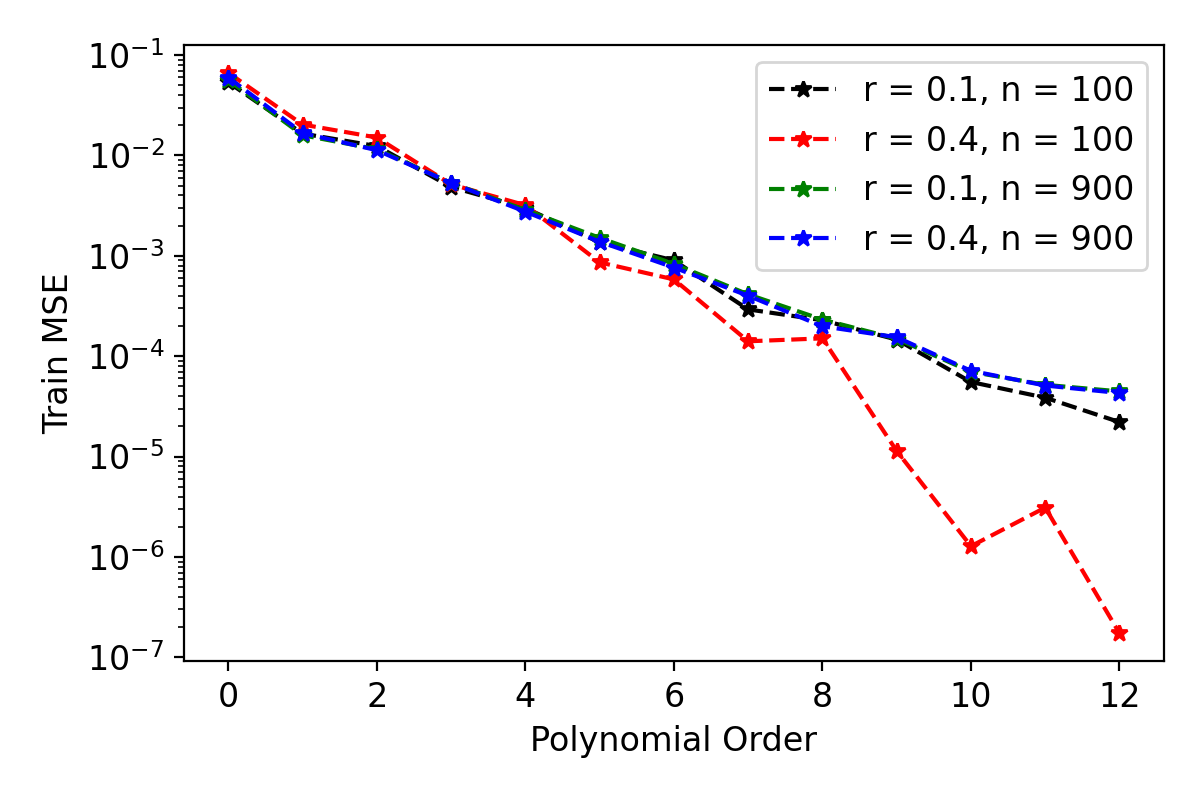
\includegraphics[width=.9\linewidth]{Images/ols2.png}
  \caption{}
  \label{fig:ols1}
\end{subfigure}%
\begin{subfigure}{.5\textwidth}
  \centering
  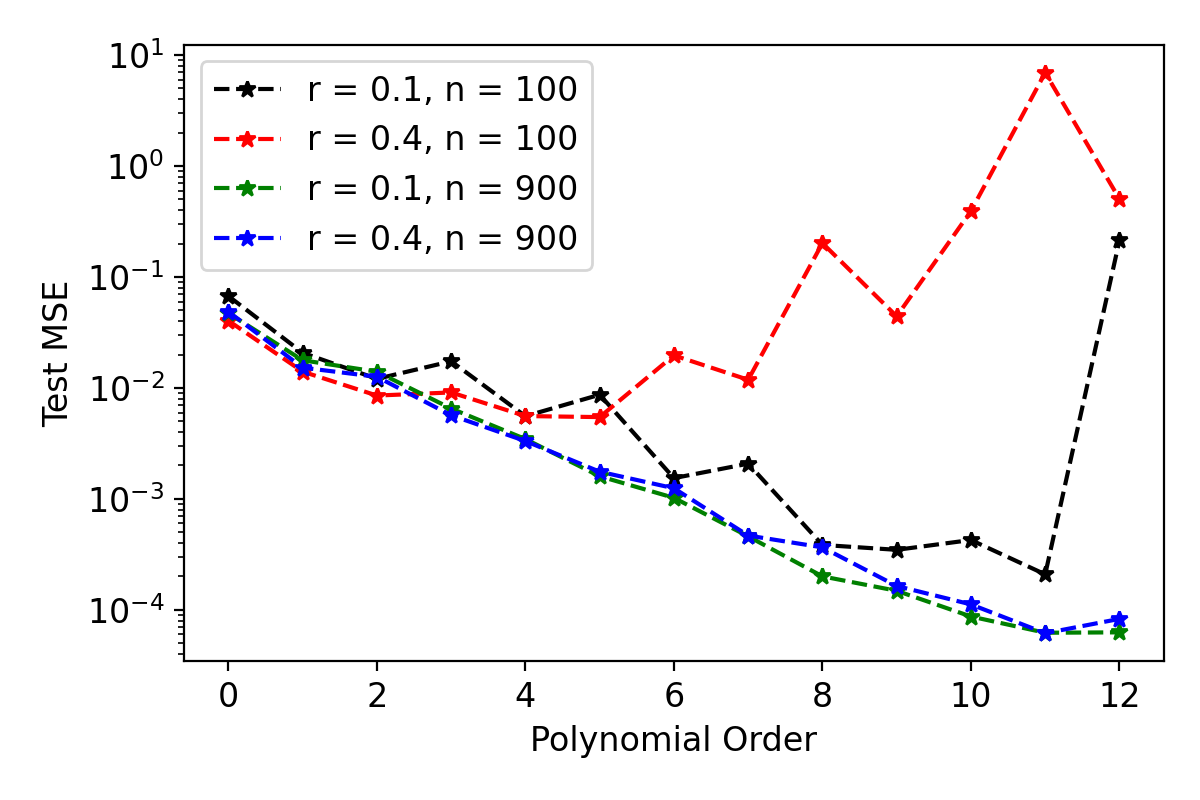
\includegraphics[width=.9\linewidth]{Images/ols1.png}
  \caption{}
  \label{fig:ols2}
\end{subfigure}
\begin{subfigure}{.5\textwidth}
  \centering
  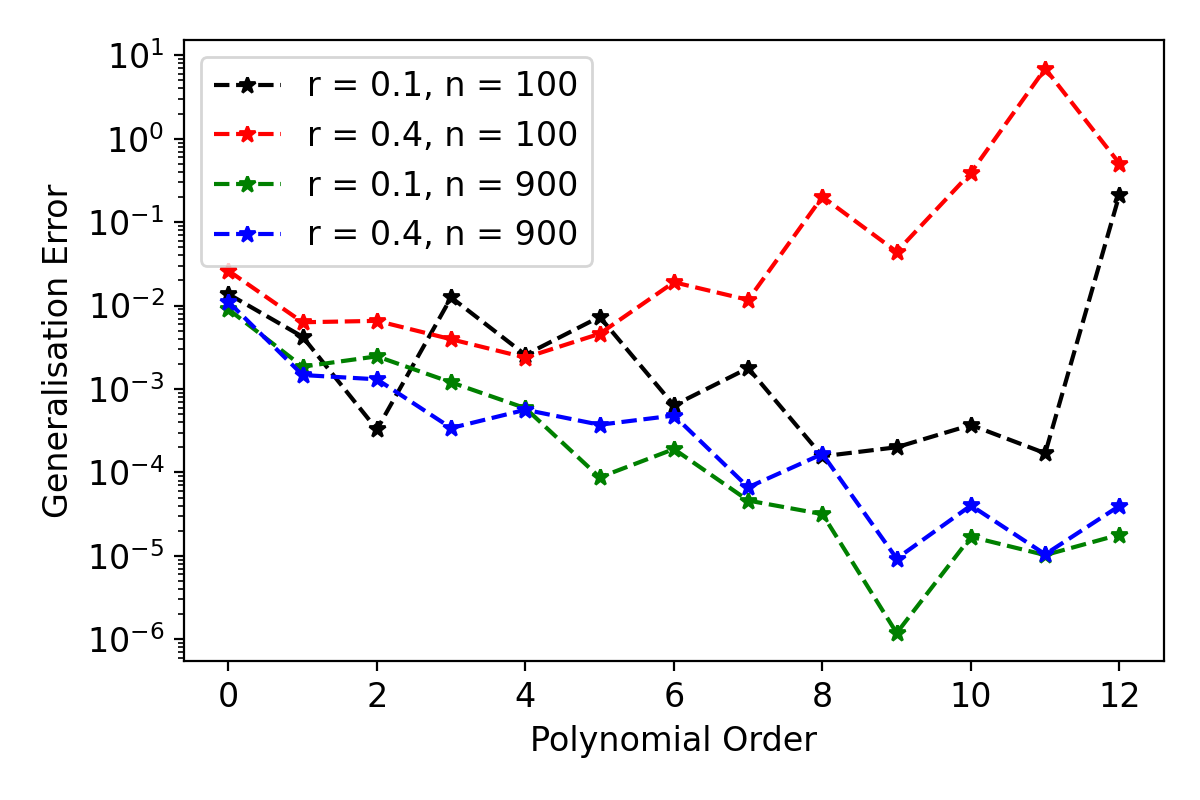
\includegraphics[width=.9\linewidth]{Images/ols3.png}
  \caption{}
  \label{fig:ols3}
\end{subfigure}
\caption{OLS for noiseless Franke data: (a) $MSE_{train}$, (b) $MSE_{test}$ and (c) Generalisation error plotted as functions of model complexity}
\label{fig:OLS1}
\end{figure}

Now, if we shift attention to the $MSE_{test}$, we see that for r=0.4, n=100, the generalisation is poor(see figure \ref{fig:ols2}). This is the result of overfitting. This also happens for r=0.4, n=100 albeit not as strongly. This shows even for low values of $MSE_{train}$, the model can perform poorly. We see that if the number of datapoints is higher in the training set, then there is no overfitting. This is also evident by looking at the generalisation error(see figure \ref{fig:ols2}). The model 'sees' more variety of data which prevents it from overfitting. Provided we don't overfit, the $MSE_{test}$ reduces as p  increases. It should be noted that irrespective of number of data points used for training, there exists p where we will experience overfitting. If $n_{train}$ is the number of training data points then to prevent overfitting, we need $n_{train} >> p$.

Next, we see that introduction of noise into the dataset increases $MSE_{train}$(see figure \ref{fig:ols4}). We also see that introduction of noise affects the $MSE_{test}$ of dataset with larger number of points significantly when model complexity is high(see figure \ref{fig:ols5}). $MSE_{test}$ decreases initially with model complexity but later plateaus. This indicated that the higher degree of freedom introduced by additional polynomial terms doesn't sufficently capture the noise. When the model complexity is low, the prediction is unaffected by the presence of noise. 

\begin{figure}
\centering
\begin{subfigure}{.5\textwidth}
  \centering
  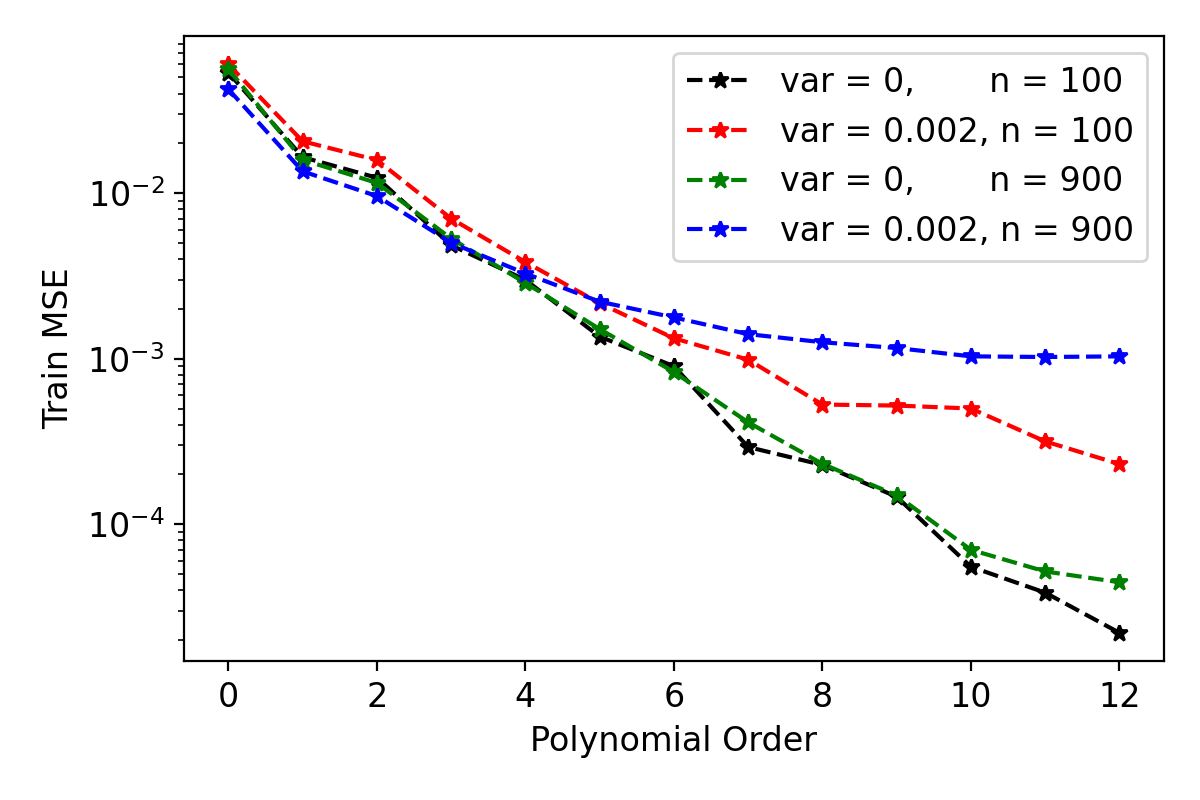
\includegraphics[width=.9\linewidth]{Images/ols5.png}
  \caption{}
  \label{fig:ols4}
\end{subfigure}%
\begin{subfigure}{.5\textwidth}
  \centering
  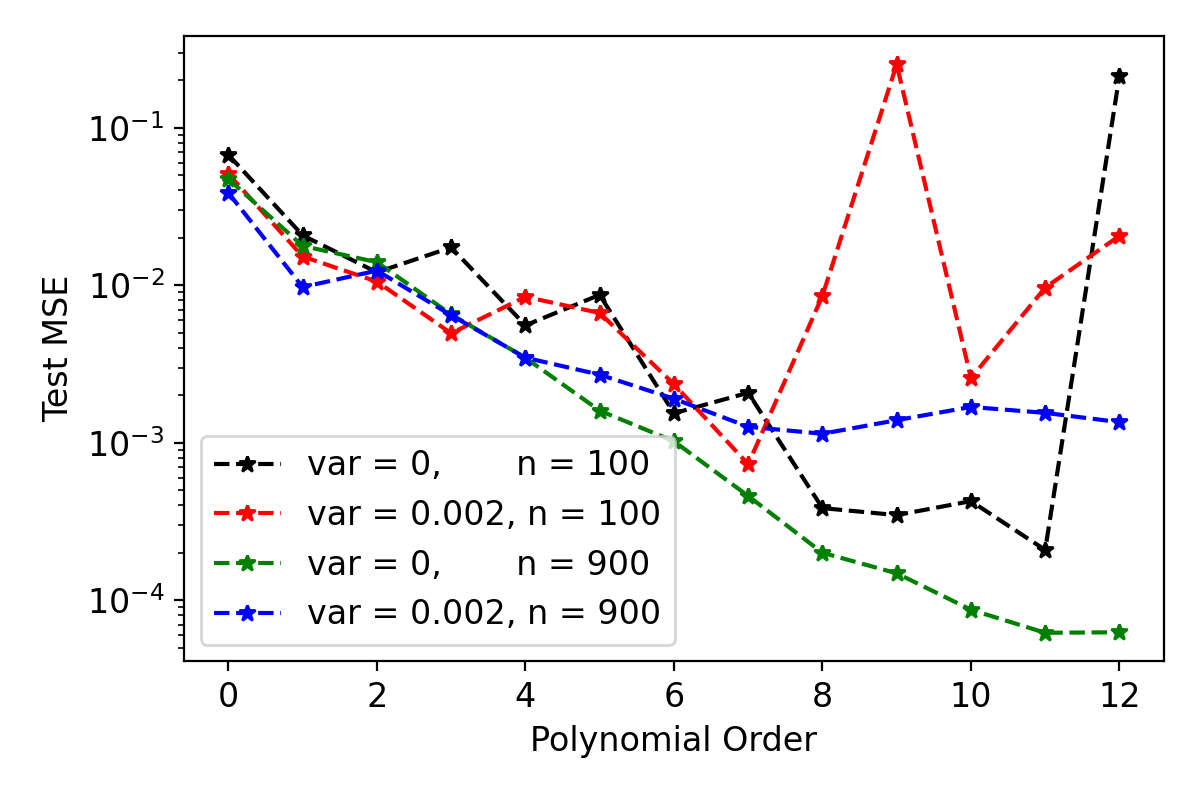
\includegraphics[width=.9\linewidth]{Images/ols4.png}
  \caption{}
  \label{fig:ols5}
\end{subfigure}
\caption{OLS for $r=0.1$ and $n=900$: (a) $MSE_{train}$ and (b) $MSE_{test}$ plotted as functions of model complexity}
\label{fig:OLS2}
\end{figure}

\begin{figure}
\centering
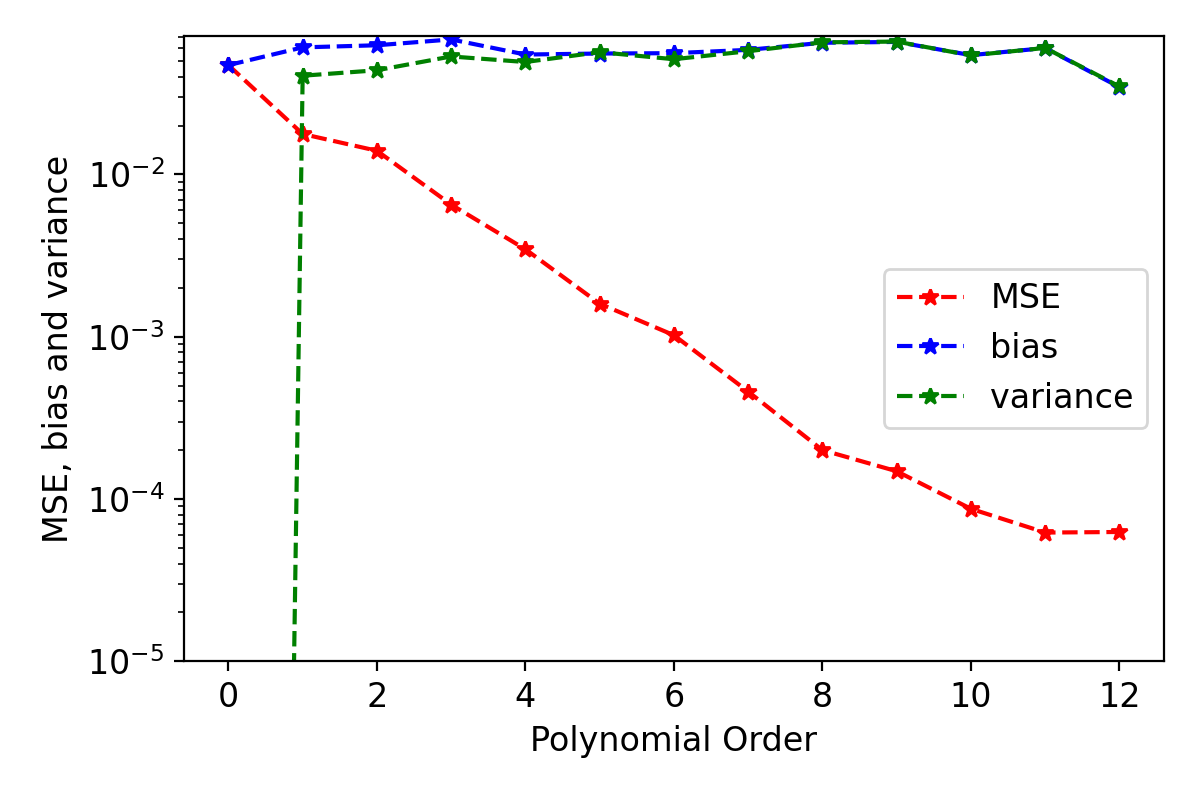
\includegraphics[width=.7\linewidth]{Images/ols7.png}
\caption{OLS for $r=0.1$, $var=0$ and $n=900$. Bias and variance plotted as functions of model complexity}
\label{fig:OLS3}
\end{figure}

If we now look at bias and variance, they are both roughly constant as the model complexity increases(see figure \ref{fig:OLS3}. This prevents us from understanding the bias-variance tradeoff. This behaviour is observed even when other parameters are changed. Variance measures the spread of our prediction, and the plots show that our model always has a finite spread. As bias is a measure of mean deviation of our prediction from the truth, the constant values raise question on our calculations. We know that parameters like $r$, $var$, $p$ and $n$ has an impact on the $MSE_{test}$, but as the bias seems to be roughly the same then that shows that irrespective of the parameters, our model has approximately the same mean value of the predicted output. Either our model is capturing the mean well almost always or our calculations of bias and variance are incorrect.

\subsubsection{Ridge and LASSO Regression}
In ridge regression, we penalise the $L_2$ norm of the parameter vector $\boldsymbol \beta$. As we are not tuning the size of the elements of the design matrix, the interrelations between the different columns should remain same. This is definitely the case when the design matrix is orthogonal. As we use polynomials as basis functions, the columns of the design matrix are likely to be independent. They will not be independent if there is a correlation between $x_{i1}$ and $x_{i2}$. This is definitely not the case for our dataset. So, the parameters in ridge regression would be rescaled by a factor of $\frac{1}{1+\lambda_r}$ compared to the OLS parameters\cite{mehta_high-bias_2019}. However, due to the fact that there might be errors in calculating the pseudoinverse, the scaling might not always be by the factor of $\frac{1}{1+\lambda_r}$. So, not all parameters are scaled the same. This would deviate the predictions from that of the OLS. We can see this in the figure \ref{fig:ridge7} and \ref{fig:ridge7b} where the regularisation parameter has an effect on both the training and prediction phase. The training and testing error both worsen as $\lambda_r$ increases. The deviation from the OLS errors kicks in at a lower model complexity for higher values of  $\lambda_r$



\begin{figure}
\centering
\begin{subfigure}{.5\textwidth}
  \centering
  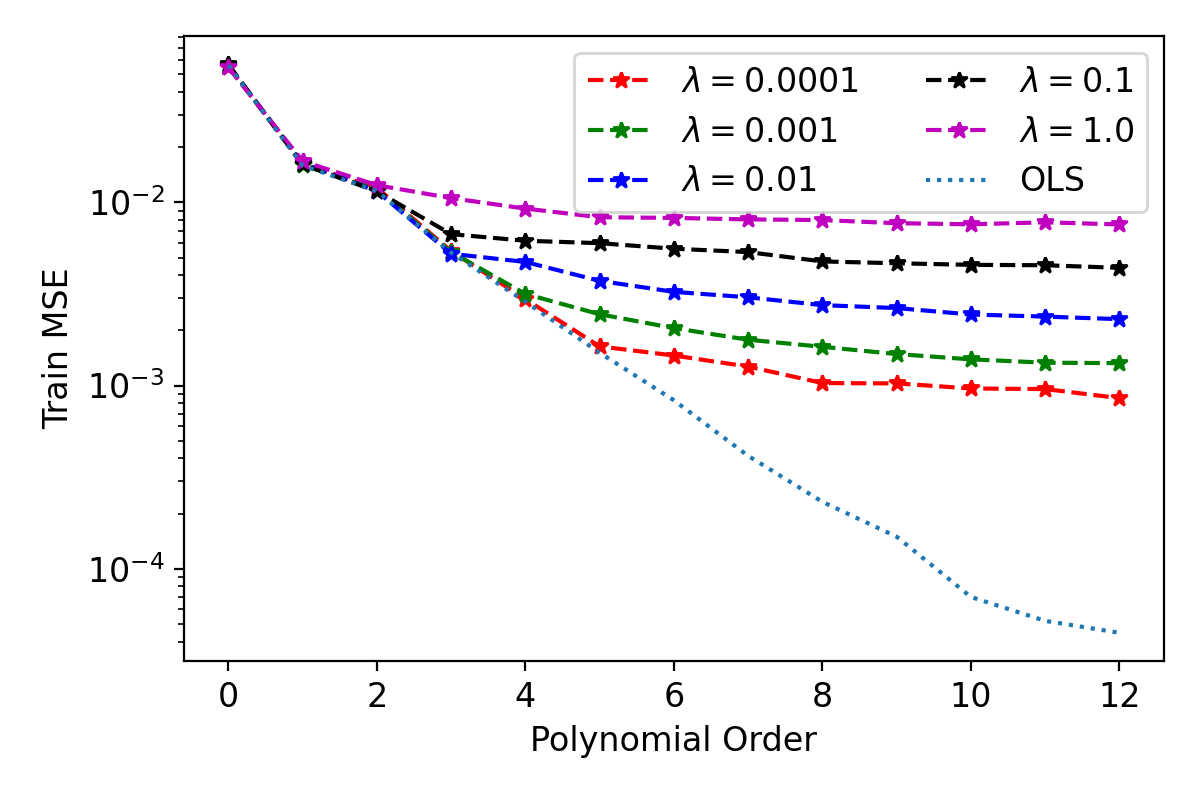
\includegraphics[width=.9\linewidth]{Images/ridge7b.png}
  \caption{}
  \label{fig:ridge7}
\end{subfigure}%
\begin{subfigure}{.5\textwidth}
  \centering
  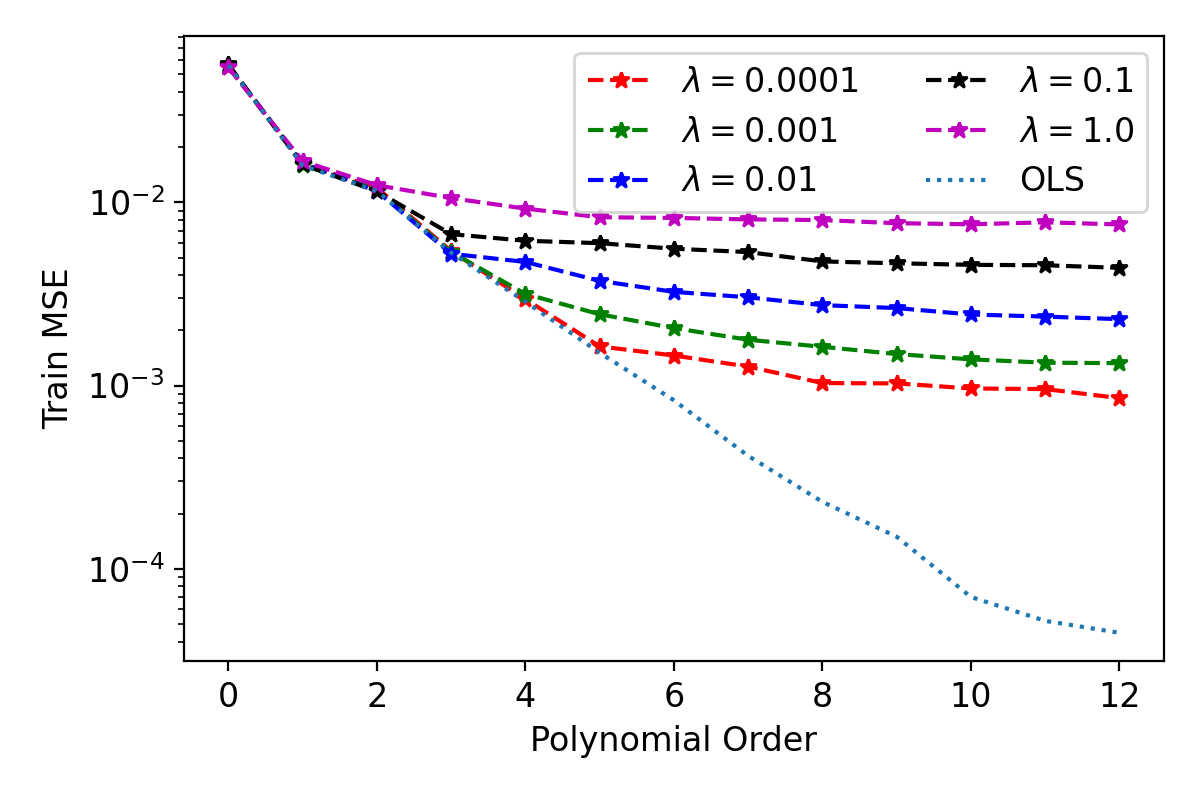
\includegraphics[width=.9\linewidth]{Images/ridge7b.png}
  \caption{}
  \label{fig:ridge7b}
\end{subfigure}
\caption{Ridge regression for $r=0.1$, $var=0$ and $n=900$: (a) $MSE_{train}$ and (b) $MSE_{test}$ plotted as functions of model complexity for different regularisation strength}
\label{fig:Ridge1}
\end{figure}

Meanwhile, in LASSO regression, we penalise the $L_1$ norm of the parameter vector $\boldsymbol \beta$. Visually, this is equivalent to optimising the parameters until we hit the edges of a hypercuboid. While, in ridge regression, we hit the surface of a hyperellipsoid. See \cite{mehta_high-bias_2019} for more details. This means that in LASSO regression, when the optimum parameters are reached, the components of some of the parameter vector $\boldsymbol \beta$ are 0. These features were not important enough in affecting the combined optimisation of the least square error and the $L_1$ norm of the parameter vector $\boldsymbol \beta$. We see in the figure \ref{fig:lasso7} that both the training error and testing error  worsen as the $\lambda_l$ increases. But, the performance is much worse than for ridge regression. As $\lambda_l$ increases, more components of $\boldsymbol \beta$ turn out to be 0. 


\begin{figure}
\centering
\begin{subfigure}{.5\textwidth}
  \centering
  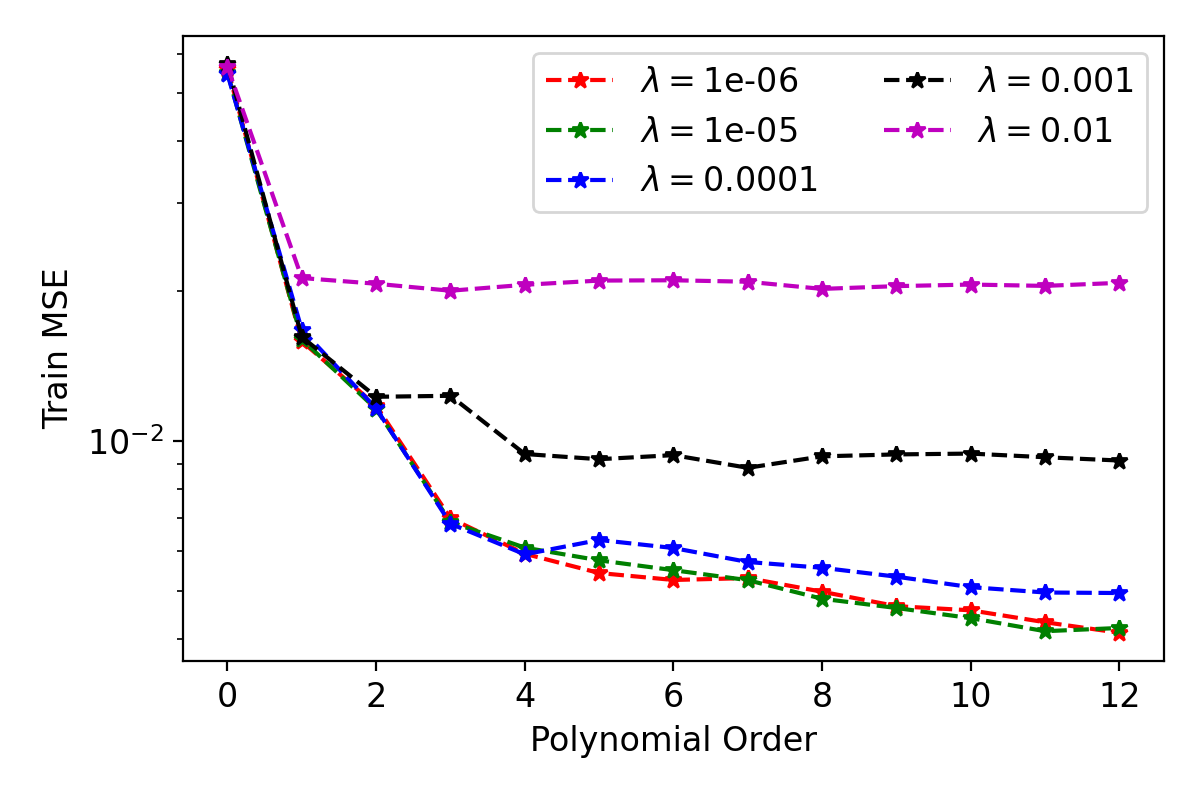
\includegraphics[width=.9\linewidth]{Images/lasso7b.png}
  \caption{}
  \label{fig:lasso7}
\end{subfigure}%
\begin{subfigure}{.5\textwidth}
  \centering
  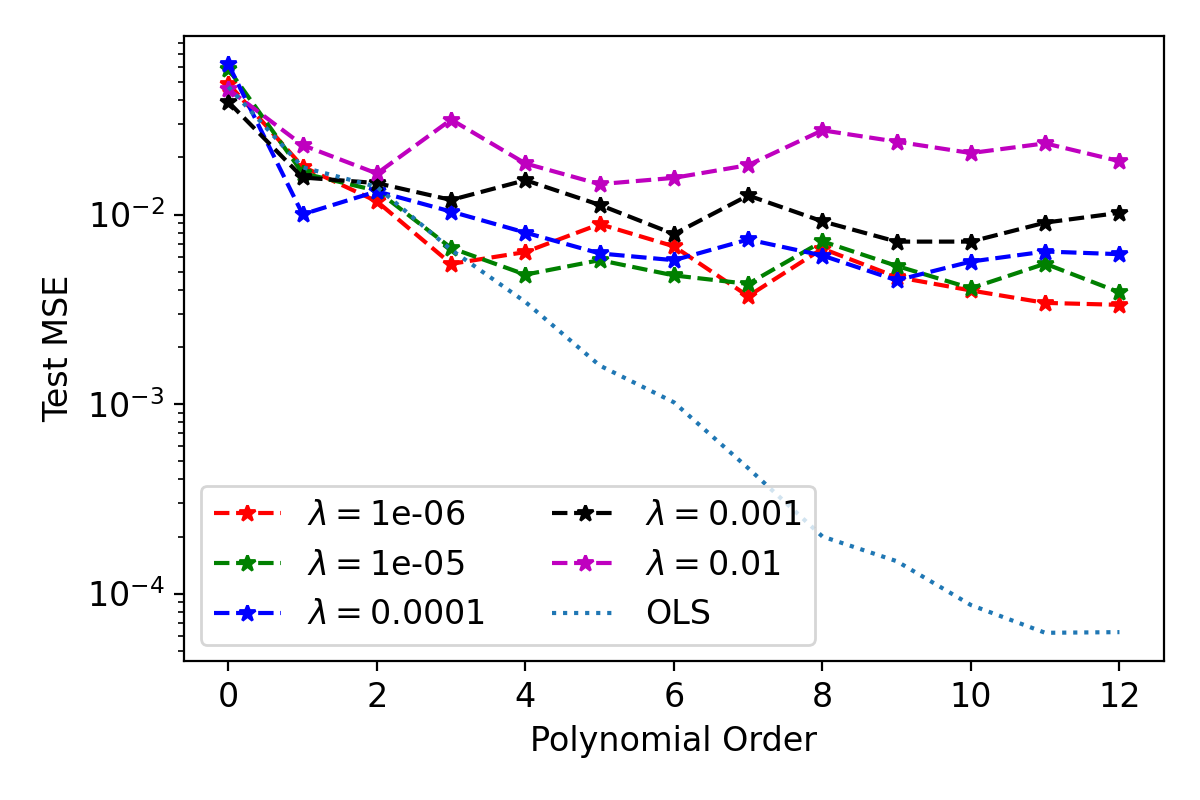
\includegraphics[width=.9\linewidth]{Images/lasso7.png}
  \caption{}
  \label{fig:lasso7b}
\end{subfigure}
\caption{LASSO regression for $r=0.1$, $var=0$ and $n=900$: (a) $MSE_{train}$ and (b) $MSE_{test}$ plotted as functions of model complexity for different regularisation strength}
\label{fig:Lasso1}
\end{figure}

\begin{figure}
\centering
\begin{subfigure}{.5\textwidth}
  \centering
  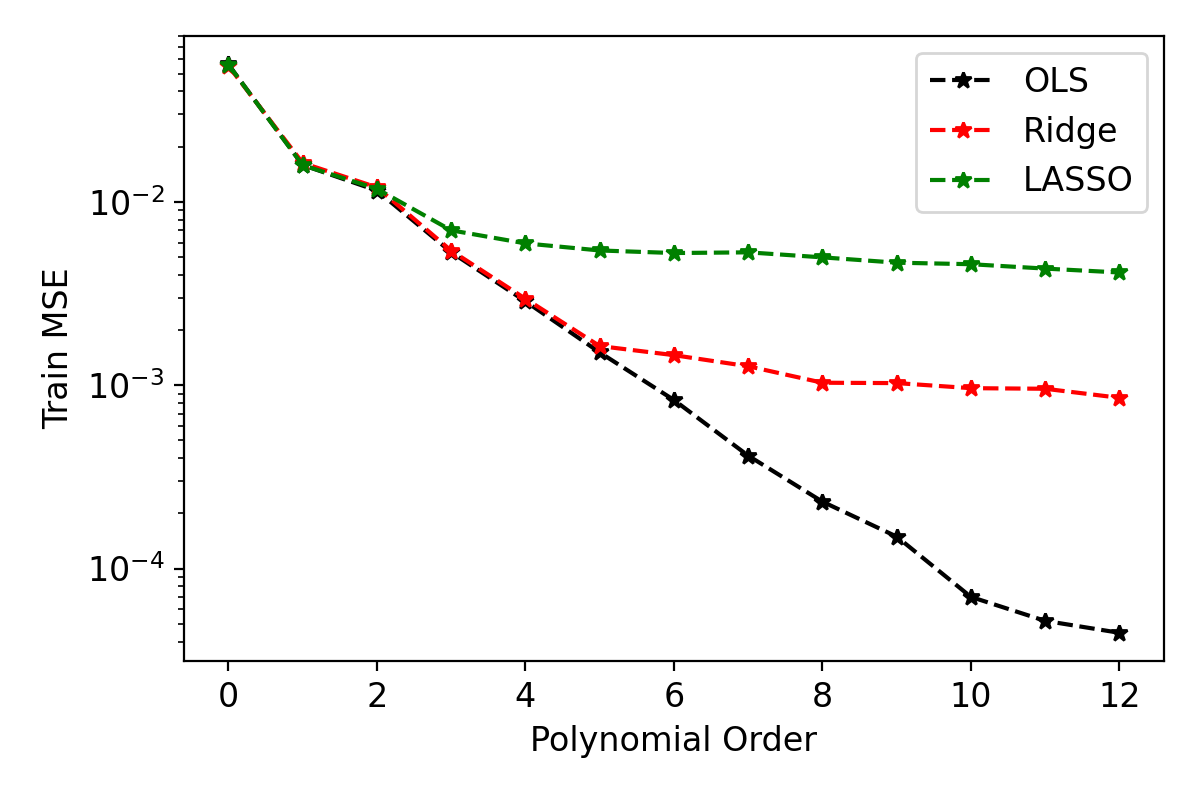
\includegraphics[width=.9\linewidth]{Images/orl2.png}
  \caption{}
  \label{fig:orl1}
\end{subfigure}%
\begin{subfigure}{.5\textwidth}
  \centering
  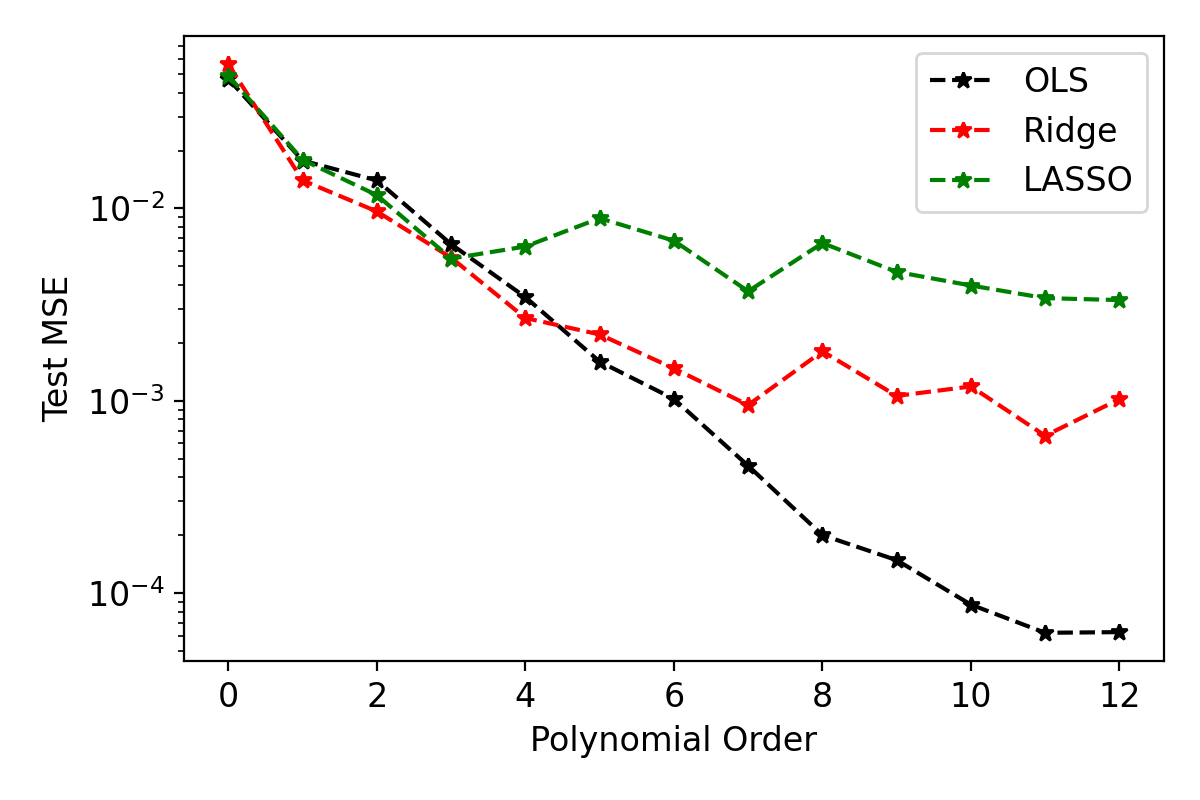
\includegraphics[width=.9\linewidth]{Images/orl1.png}
  \caption{}
  \label{fig:orl2}
\end{subfigure}
\begin{subfigure}{.5\textwidth}
  \centering
  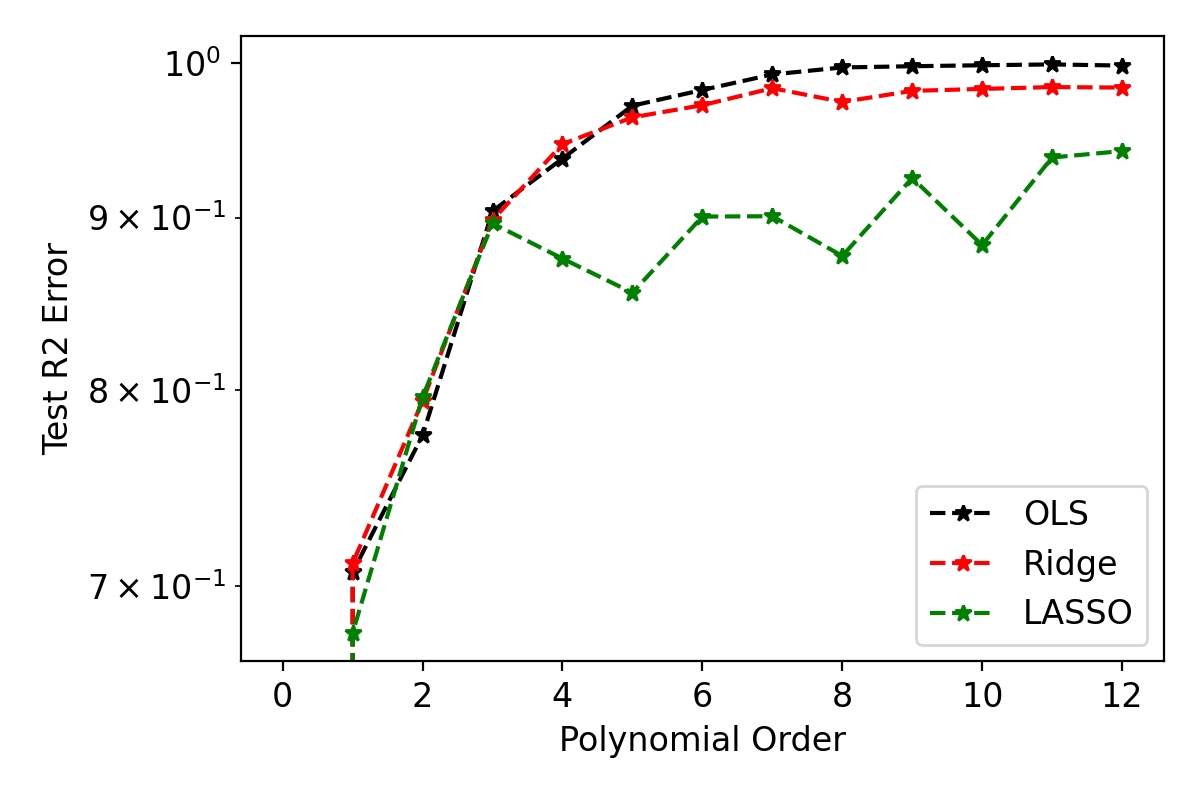
\includegraphics[width=.9\linewidth]{Images/orl3.png}
  \caption{}
  \label{fig:orl3}
\end{subfigure}
\caption{OLS, Ridge($\lambda_r = \num{1e-4}$) and LASSO($\lambda_l = \num{1e-6}$) regression for $r=0.1$, $var=0$ and $n=900$: (a) $MSE_{train}$, (b) $MSE_{test}$ and (c) $R^2_{test}$ plotted as functions of model complexity}
\label{fig:ORL1}
\end{figure}

\subsubsection{OLS with Bootstrap and Crossvalidation}
No difference for large n but for small n bootstrap training is better due to overfitting(due to sampling with replacement). But, testing is worse for bootstrap and for CV compared to OLS. The results of bootstrap is obvious but not that of why CV performs much worse than ols without sampling. It should be the same right?????

\begin{figure}
\centering
\begin{subfigure}{.5\textwidth}
  \centering
  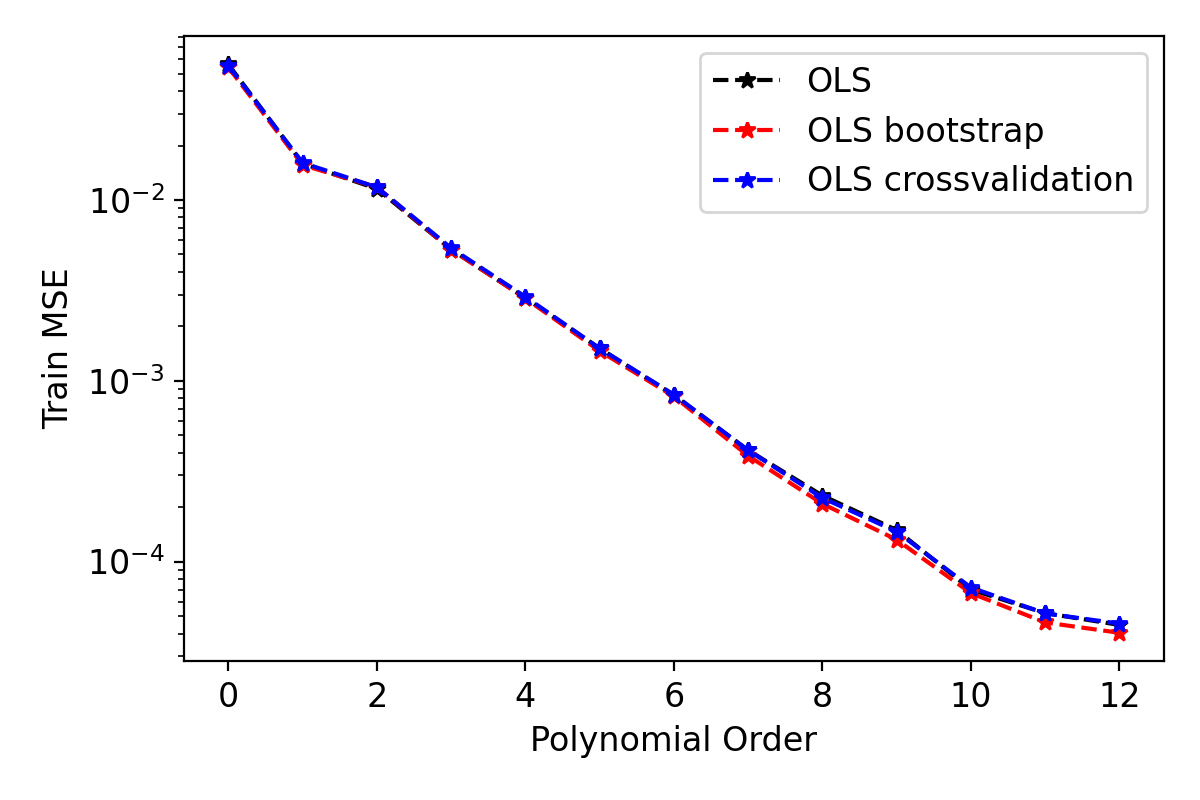
\includegraphics[width=.9\linewidth]{Images/ols9.png}
  \caption{}
  \label{fig:ols9}
\end{subfigure}%
\begin{subfigure}{.5\textwidth}
  \centering
  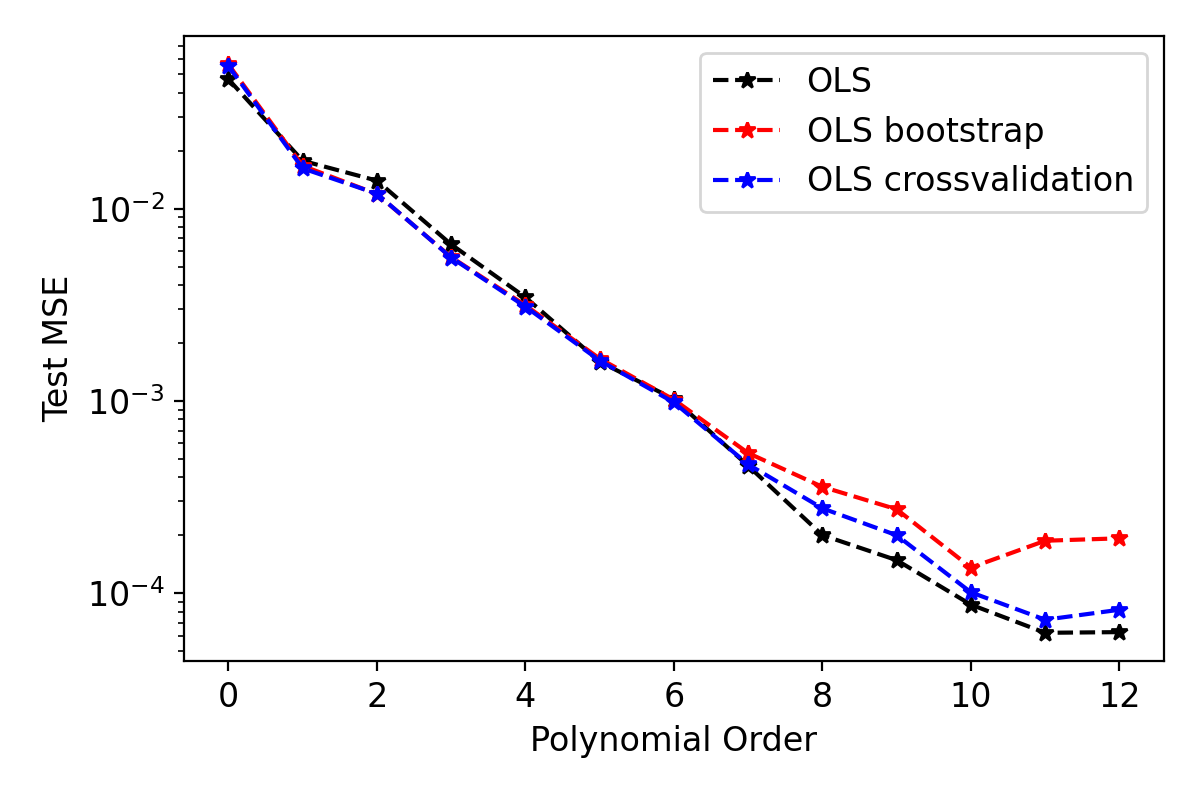
\includegraphics[width=.9\linewidth]{Images/ols8.png}
  \caption{}
  \label{fig:ols8}
\end{subfigure}
\begin{subfigure}{.5\textwidth}
  \centering
  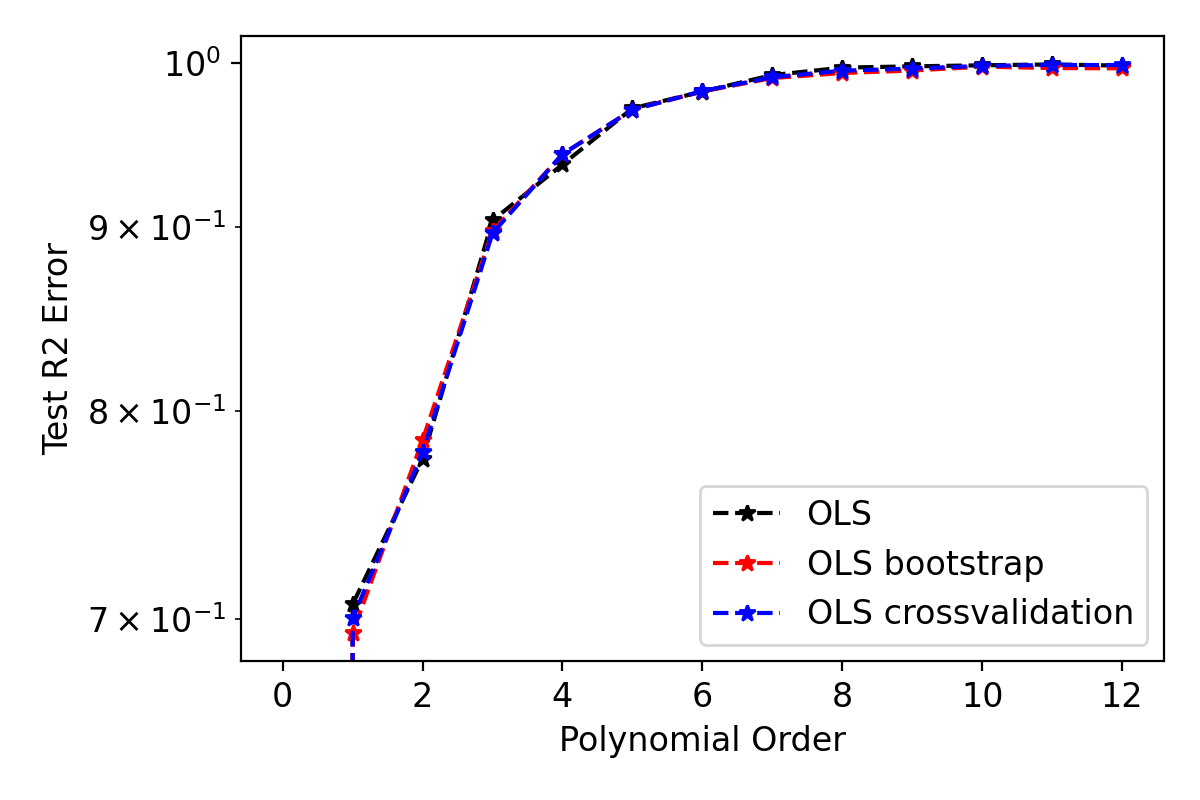
\includegraphics[width=.9\linewidth]{Images/ols10.png}
  \caption{}
  \label{fig:ols10}
\end{subfigure}
\caption{For $r=0.1$, $var=0$ and $n=900$: (a) $MSE_{train}$, (b) $MSE_{test}$ and (c) R2 error plotted as functions of model complexity}
\label{fig:OLS_resample}
\end{figure}



\begin{figure}
\centering
\begin{subfigure}{.5\textwidth}
  \centering
  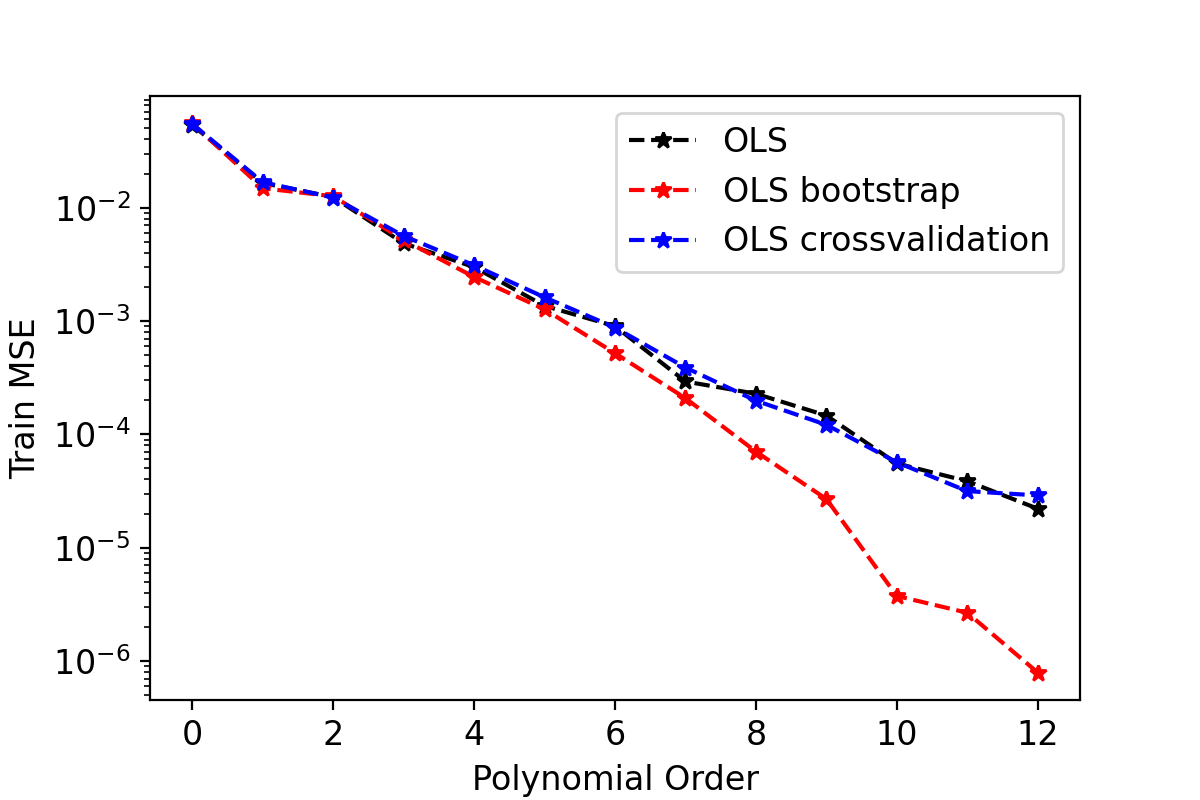
\includegraphics[width=.9\linewidth]{Images/ols15.png}
  \caption{}
  \label{fig:ols15}
\end{subfigure}%
\begin{subfigure}{.5\textwidth}
  \centering
  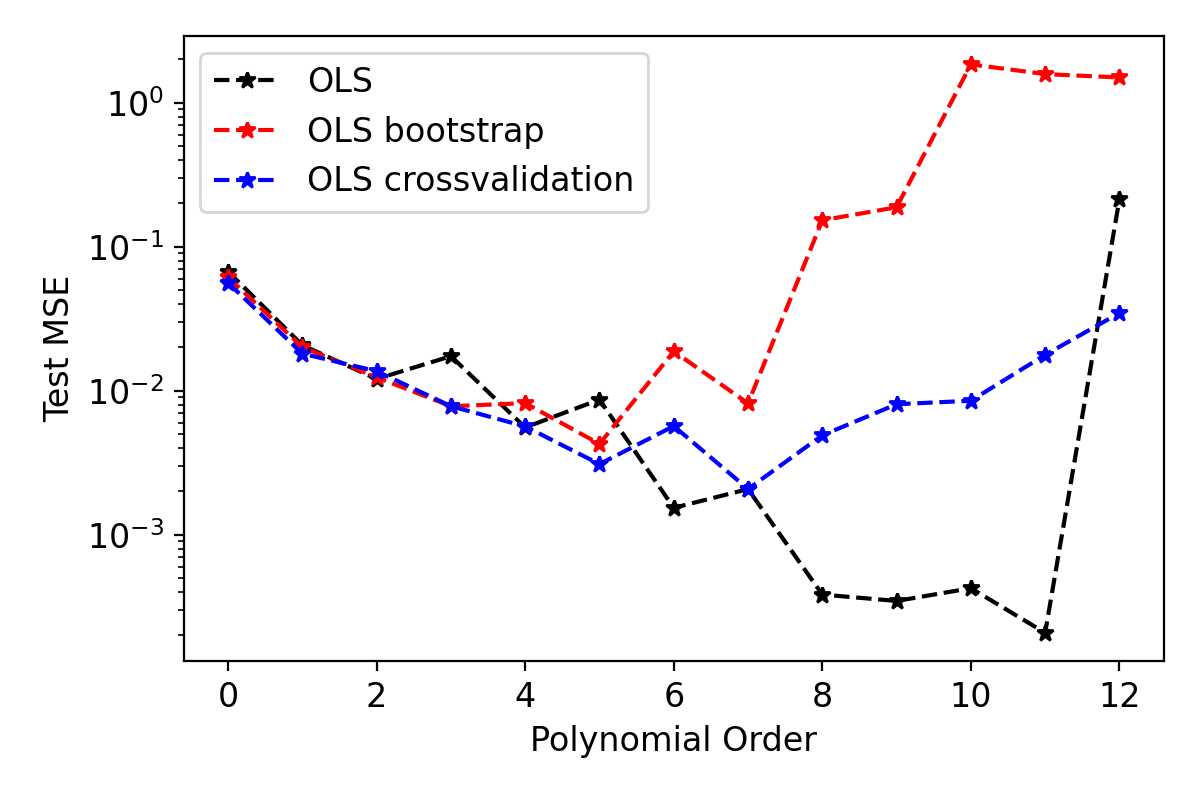
\includegraphics[width=.9\linewidth]{Images/ols14.png}
  \caption{}
  \label{fig:ols14}
\end{subfigure}
\begin{subfigure}{.5\textwidth}
  \centering
  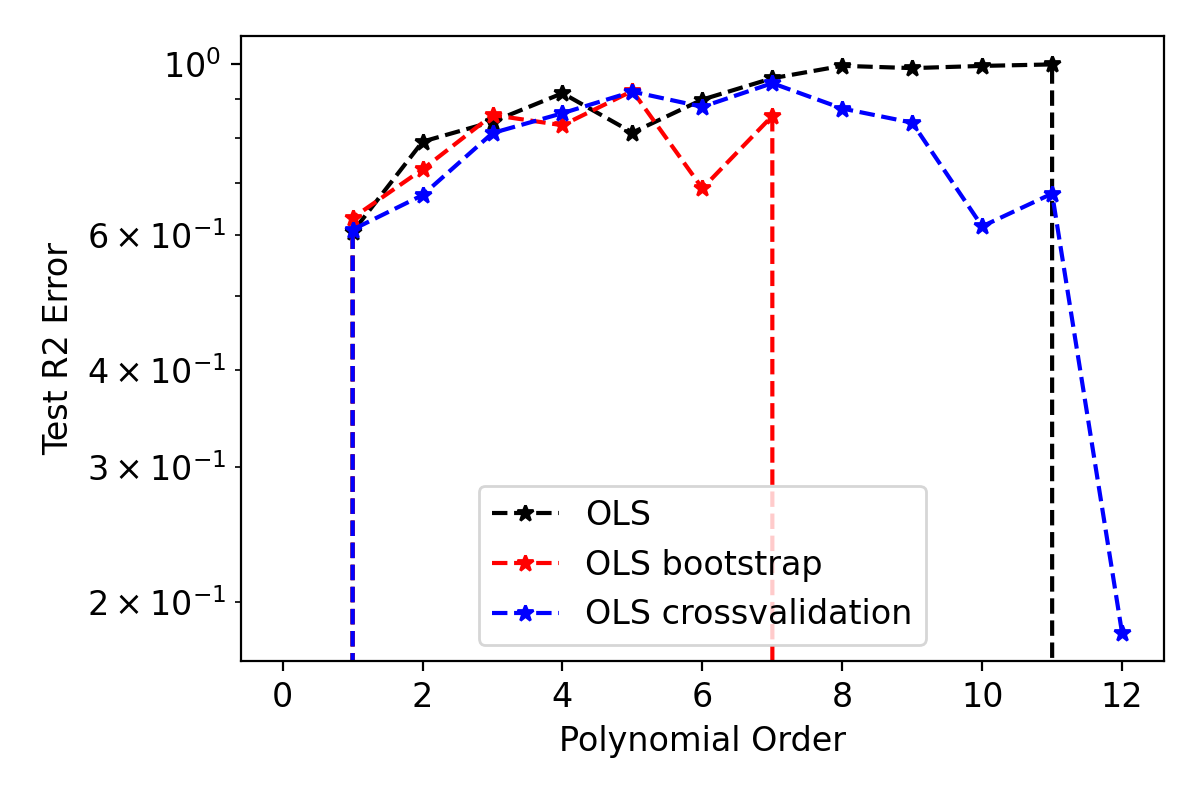
\includegraphics[width=.9\linewidth]{Images/ols16.png}
  \caption{}
  \label{fig:ols16}
\end{subfigure}
\caption{For $r=0.1$, $var=0$ and $n=100$: (a) $MSE_{train}$, (b) $MSE_{test}$ and (c) R2 error plotted as functions of model complexity}
\label{fig:OLS_resample2}
\end{figure}

\subsubsection{Ridge with Bootstrap and Crossvalidation}
No difference at all???

\begin{figure}
\centering
\begin{subfigure}{.5\textwidth}
  \centering
  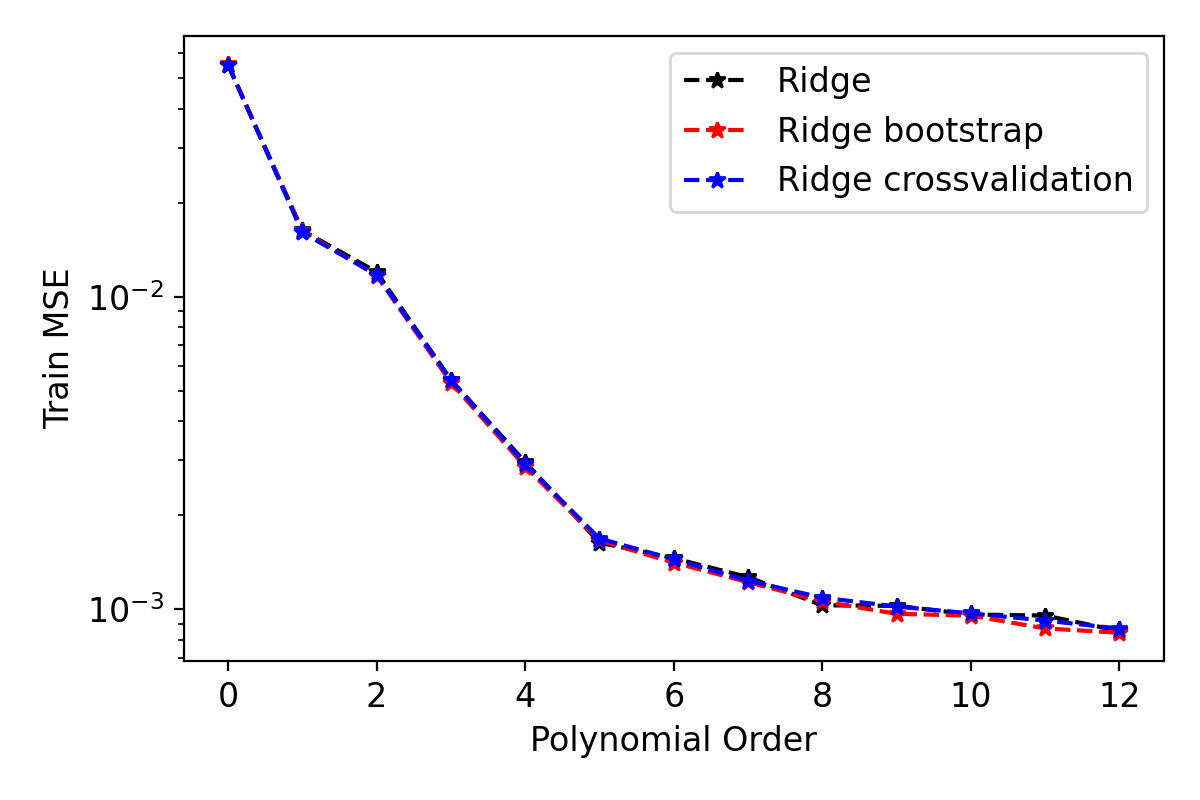
\includegraphics[width=.9\linewidth]{Images/ridge9.png}
  \caption{}
  \label{fig:ridge9}
\end{subfigure}%
\begin{subfigure}{.5\textwidth}
  \centering
  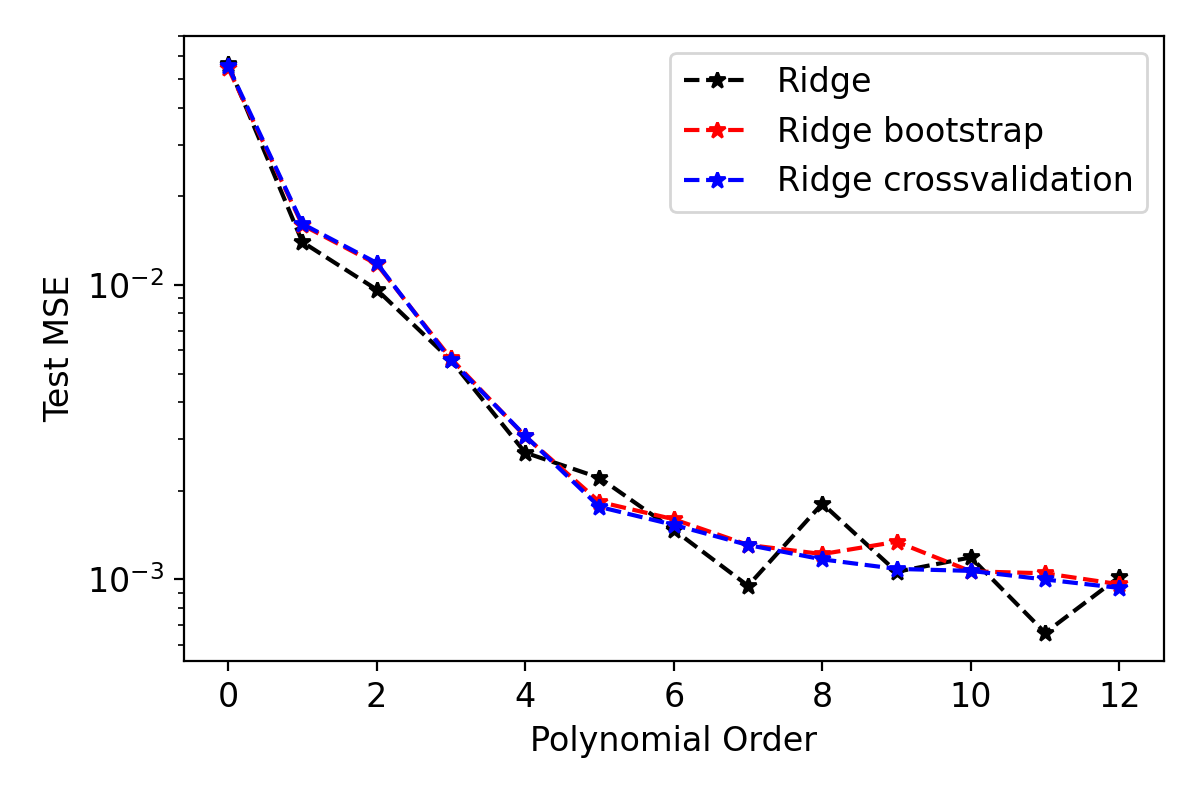
\includegraphics[width=.9\linewidth]{Images/ridge8.png}
  \caption{}
  \label{fig:ridge8}
\end{subfigure}
\begin{subfigure}{.5\textwidth}
  \centering
  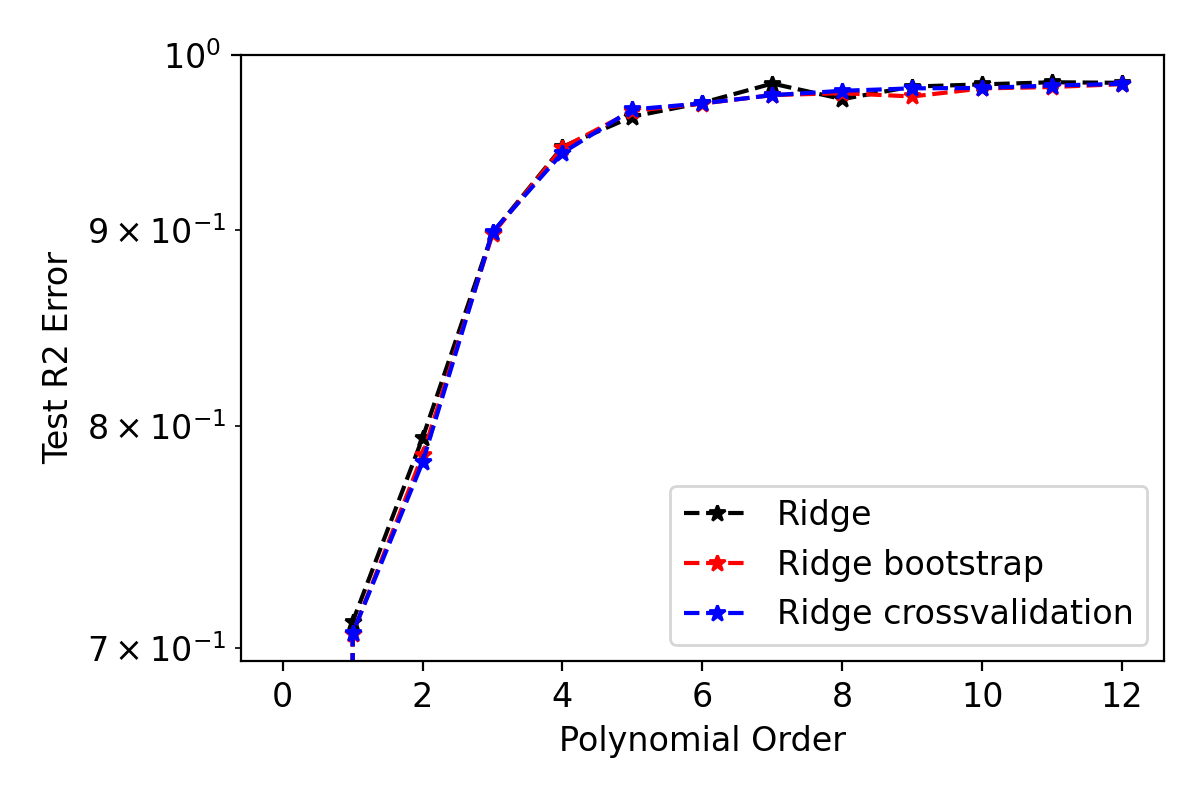
\includegraphics[width=.9\linewidth]{Images/ridge10.png}
  \caption{}
  \label{fig:ridge10}
\end{subfigure}
\caption{For $r=0.1$, $var=0$ and $n=900$: (a) $MSE_{train}$, (b) $MSE_{test}$ and (c) R2 error plotted as functions of model complexity}
\label{fig:Ridge_resample}
\end{figure}



\begin{figure}
\centering
\begin{subfigure}{.5\textwidth}
  \centering
  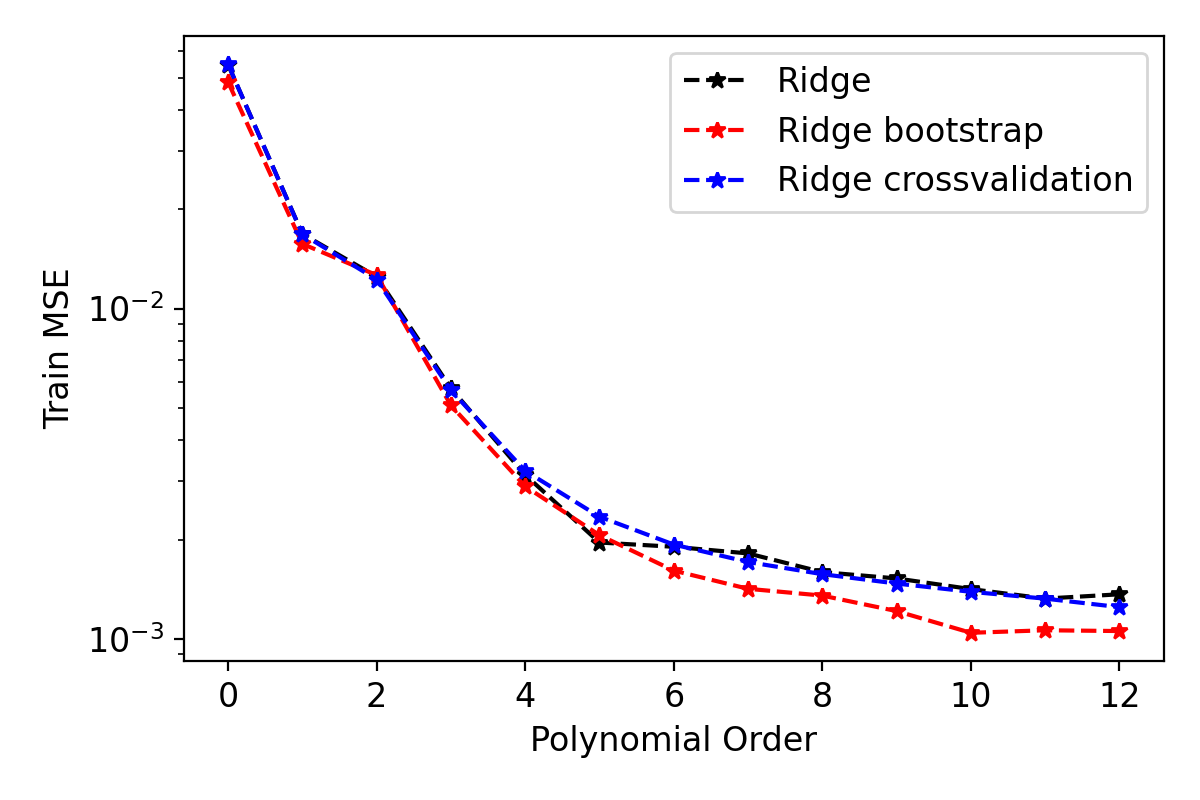
\includegraphics[width=.9\linewidth]{Images/ridge12.png}
  \caption{}
  \label{fig:ridge12}
\end{subfigure}%
\begin{subfigure}{.5\textwidth}
  \centering
  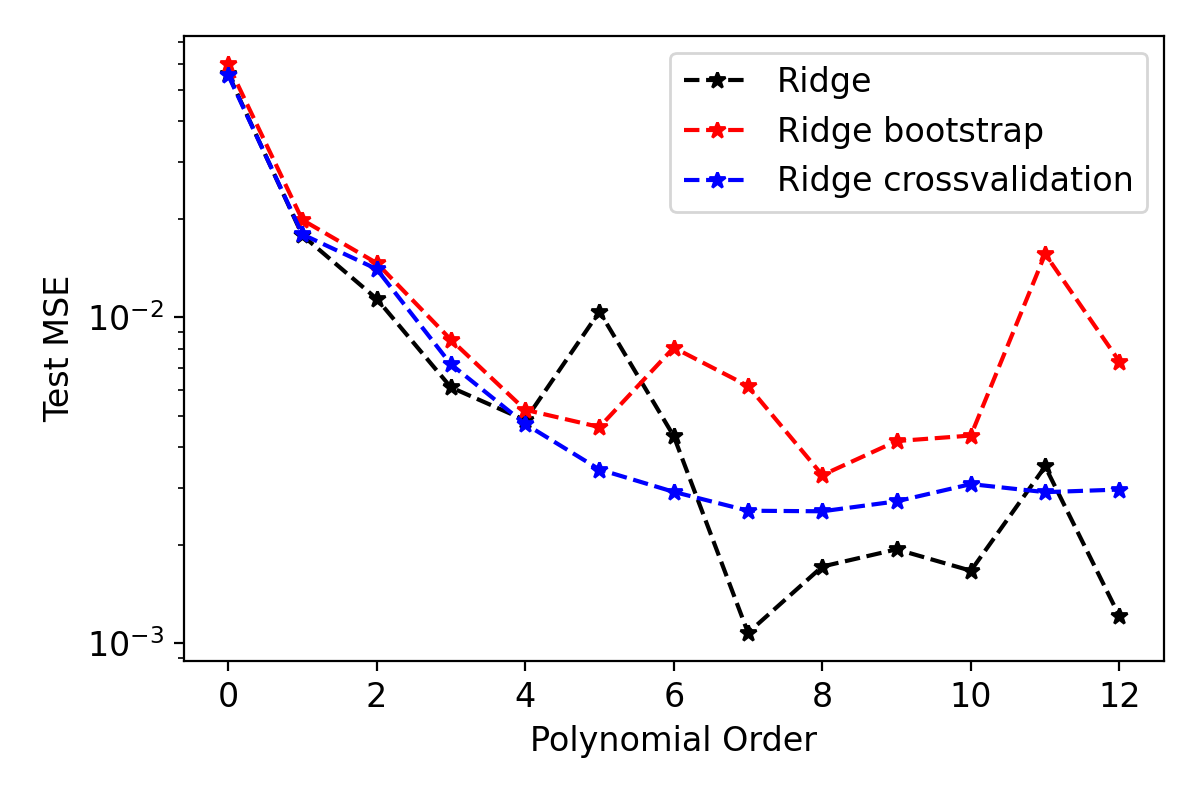
\includegraphics[width=.9\linewidth]{Images/ridge11.png}
  \caption{}
  \label{fig:ridge11}
\end{subfigure}
\begin{subfigure}{.5\textwidth}
  \centering
  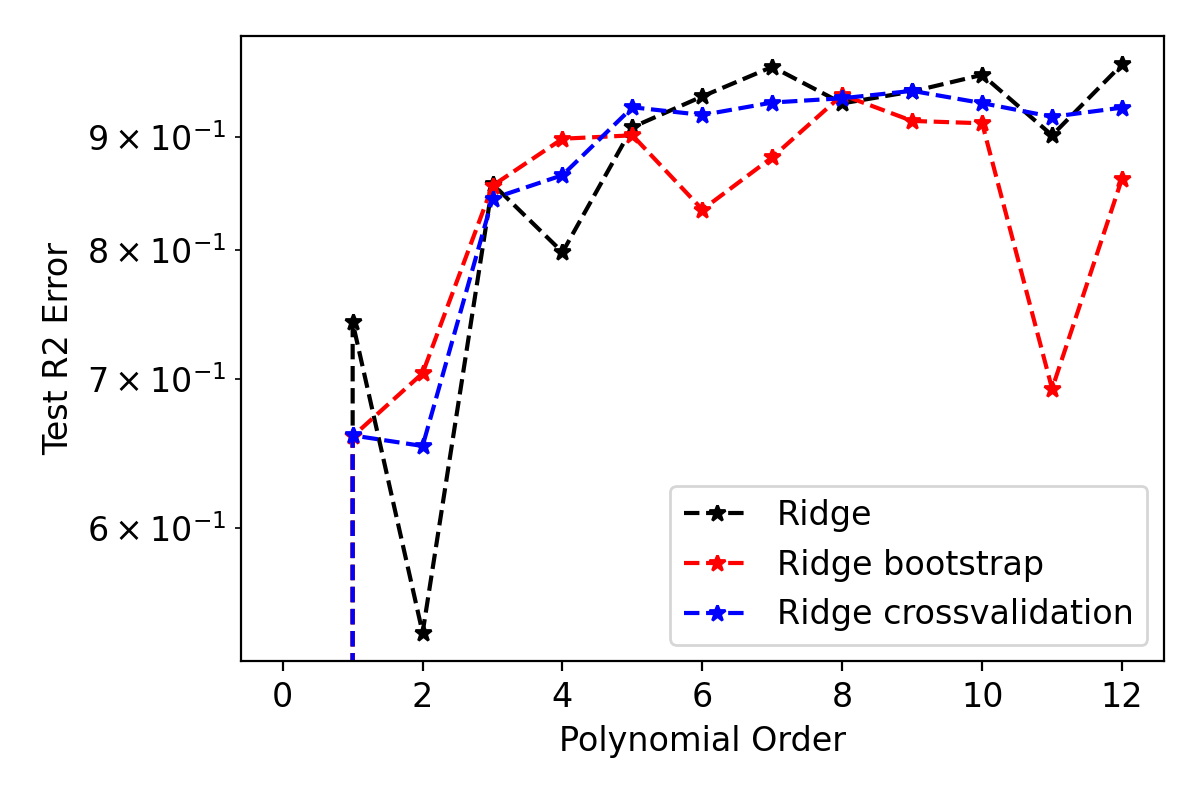
\includegraphics[width=.9\linewidth]{Images/ridge13.png}
  \caption{}
  \label{fig:ridge13}
\end{subfigure}
\caption{For $r=0.1$, $var=0$ and $n=100$: (a) $MSE_{train}$, (b) $MSE_{test}$ and (c) R2 error plotted as functions of model complexity}
\label{fig:Ridge_resample 100}
\end{figure}

\subsubsection{LASSO with Bootstrap and Crossvalidation}
No difference at all???

\begin{figure}
\centering
\begin{subfigure}{.5\textwidth}
  \centering
  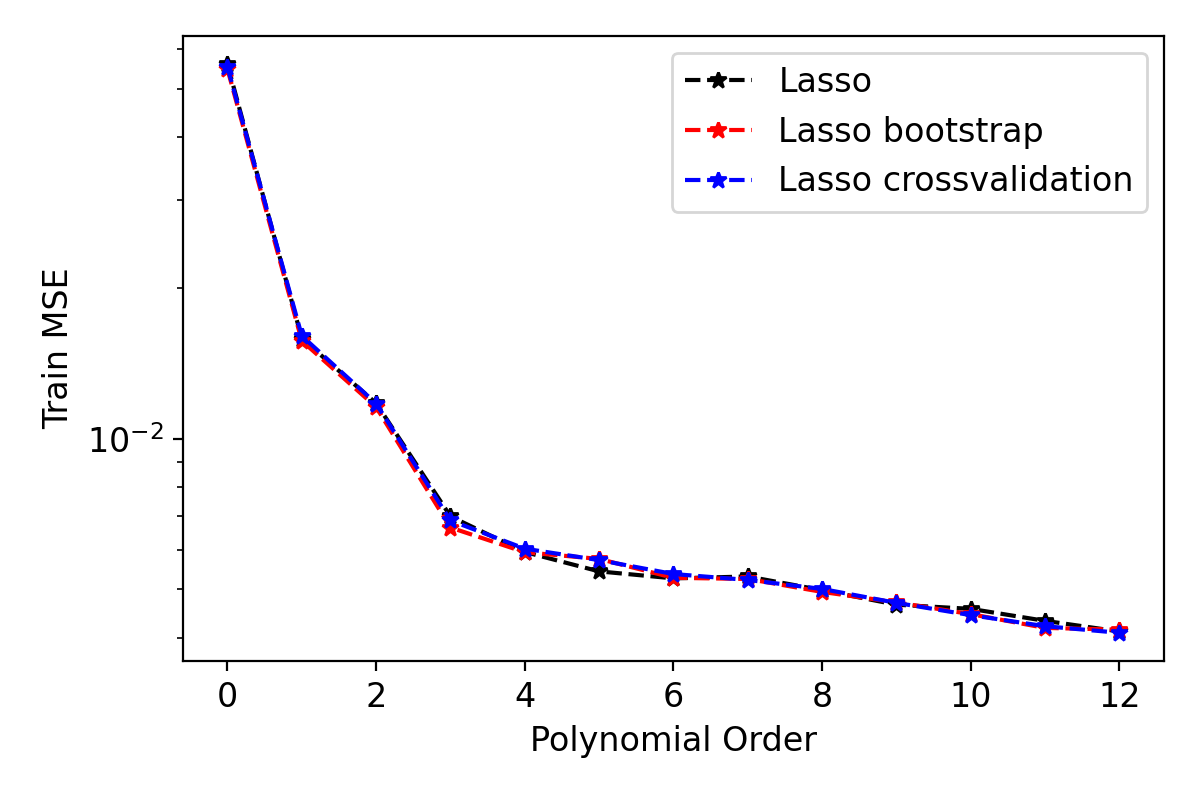
\includegraphics[width=.9\linewidth]{Images/lasso9.png}
  \caption{}
  \label{fig:lasso9}
\end{subfigure}%
\begin{subfigure}{.5\textwidth}
  \centering
  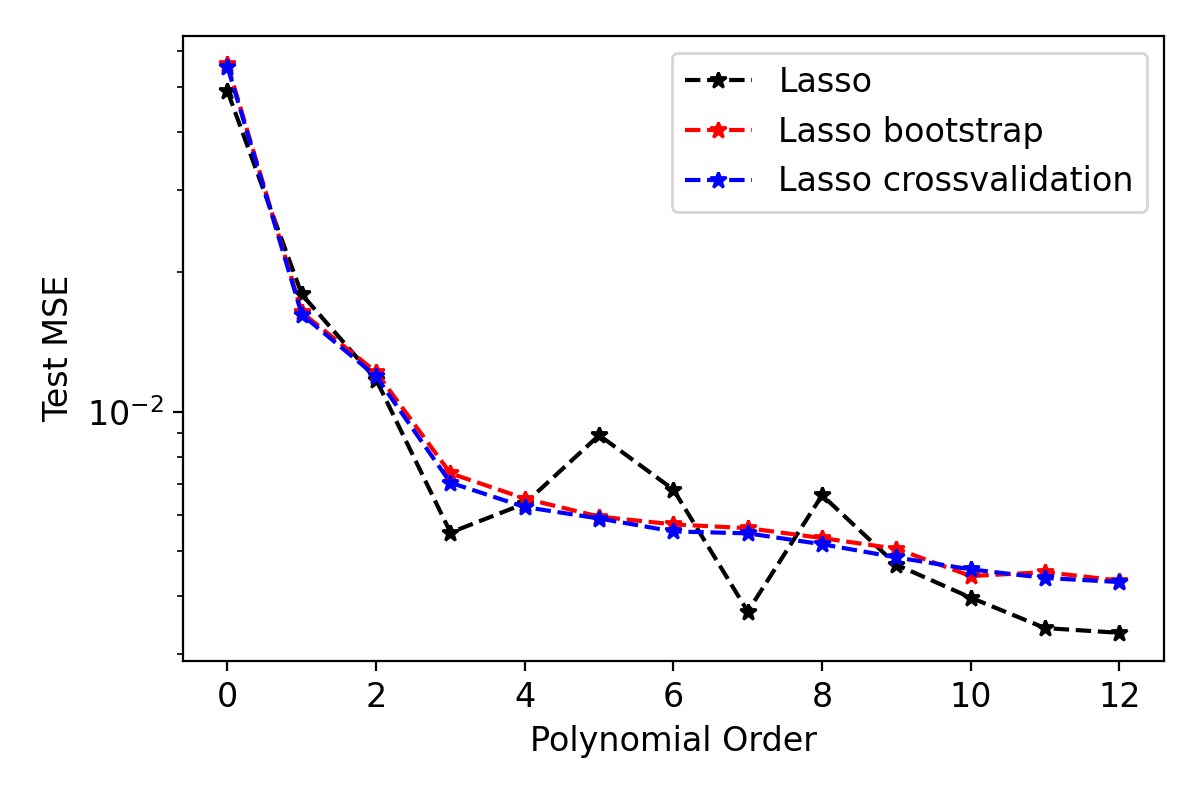
\includegraphics[width=.9\linewidth]{Images/lasso8.png}
  \caption{}
  \label{fig:lasso8}
\end{subfigure}
\begin{subfigure}{.5\textwidth}
  \centering
  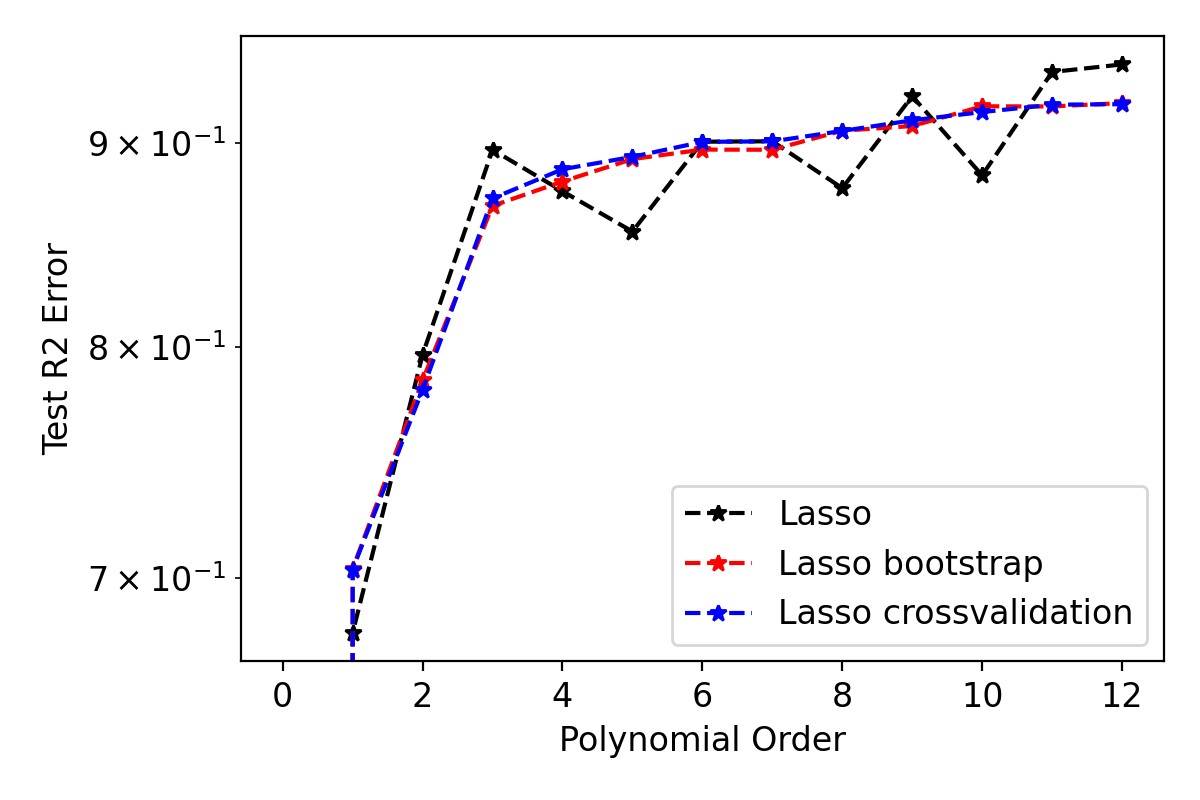
\includegraphics[width=.9\linewidth]{Images/lasso10.png}
  \caption{}
  \label{fig:lasso10}
\end{subfigure}
\caption{For $r=0.1$, $var=0$ and $n=900$: (a) $MSE_{train}$, (b) $MSE_{test}$ and (c) R2 error plotted as functions of model complexity}
\label{fig:lasso_resample}
\end{figure}



\begin{figure}
\centering
\begin{subfigure}{.5\textwidth}
  \centering
  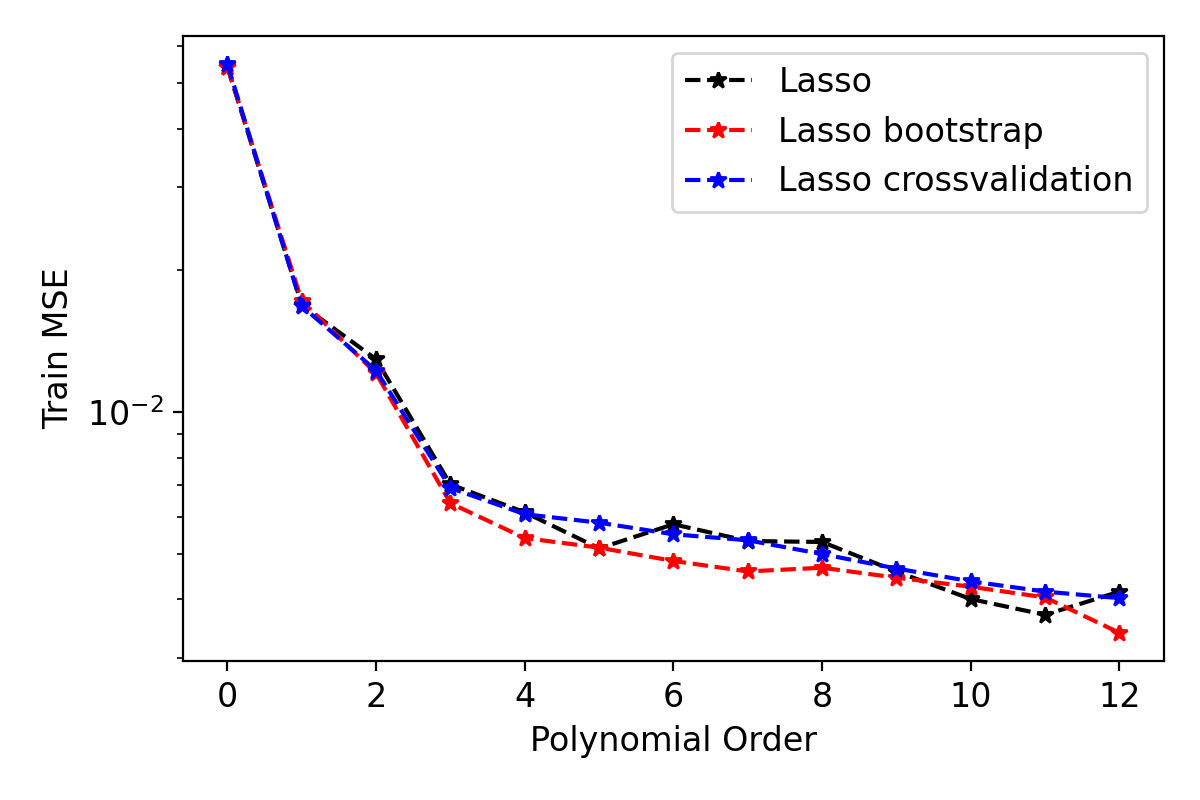
\includegraphics[width=.9\linewidth]{Images/lasso12.png}
  \caption{}
  \label{fig:lasso12}
\end{subfigure}%
\begin{subfigure}{.5\textwidth}
  \centering
  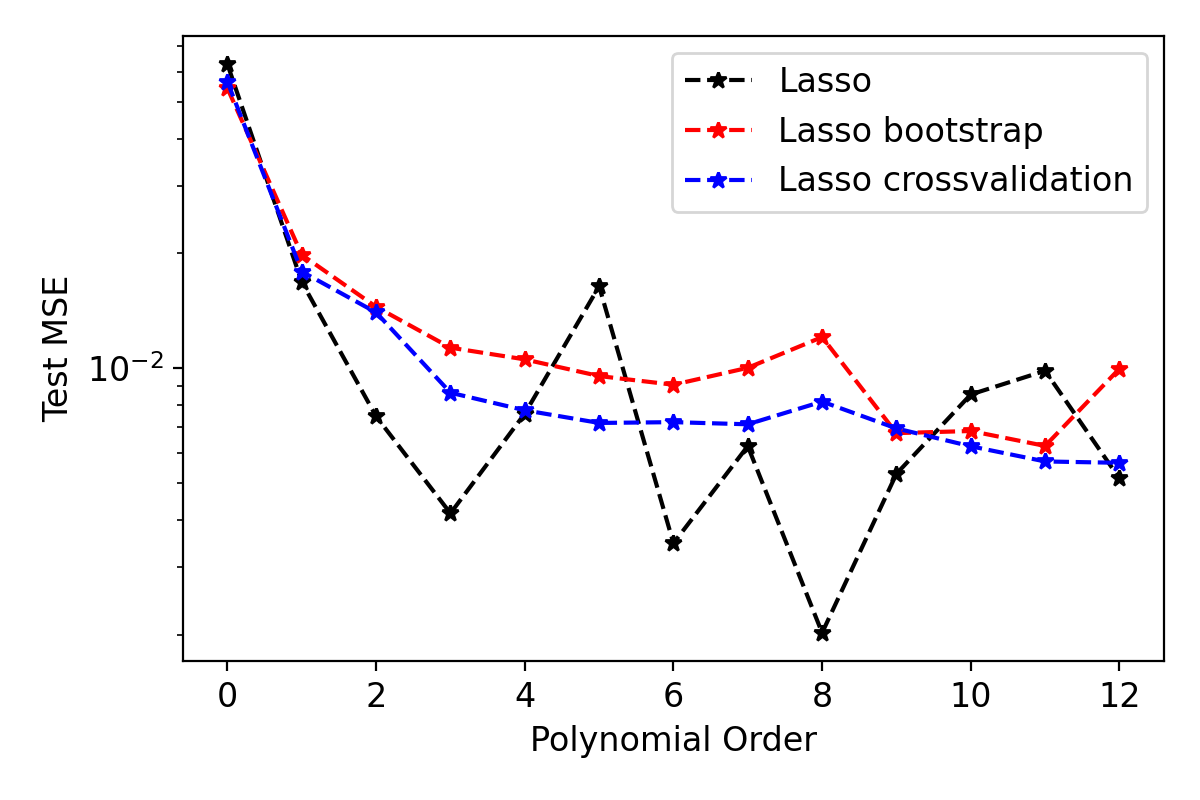
\includegraphics[width=.9\linewidth]{Images/lasso11.png}
  \caption{}
  \label{fig:lasso11}
\end{subfigure}
\begin{subfigure}{.5\textwidth}
  \centering
  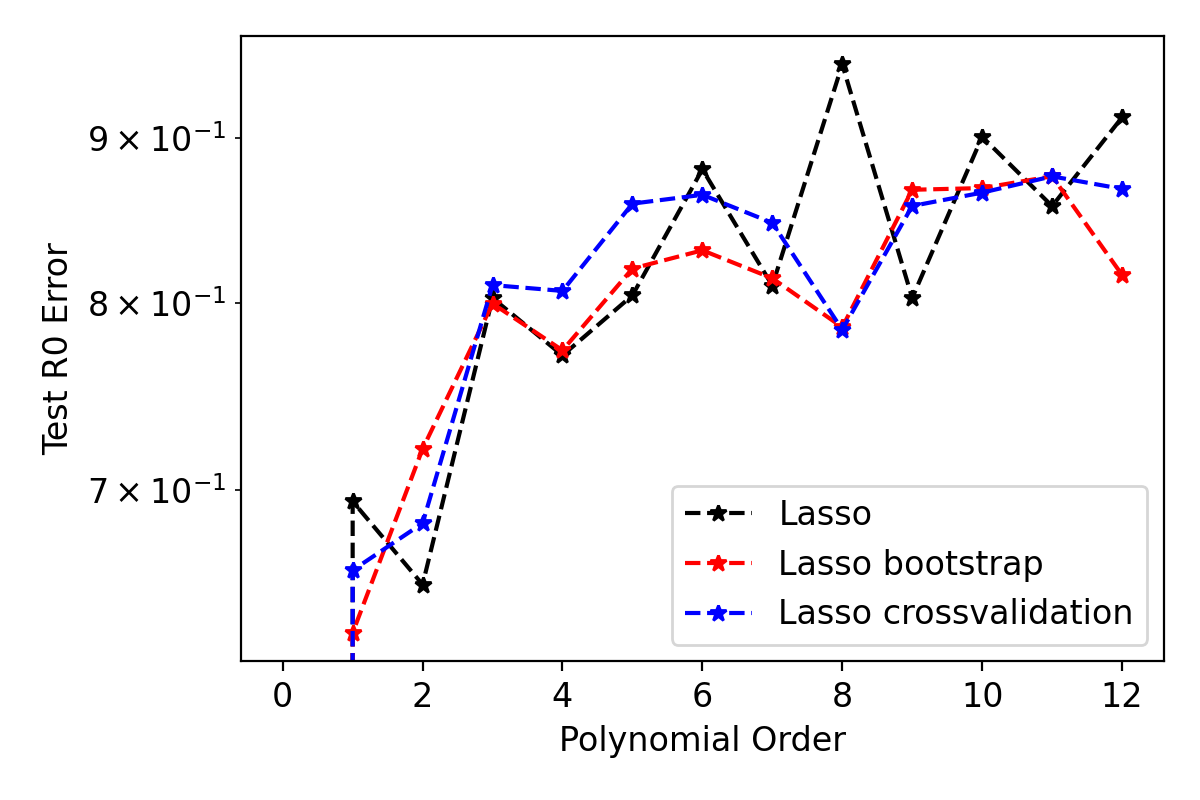
\includegraphics[width=.9\linewidth]{Images/lasso13.png}
  \caption{}
  \label{fig:lasso13}
\end{subfigure}
\caption{For $r=0.1$, $var=0$ and $n=100$: (a) $MSE_{train}$, (b) $MSE_{test}$ and (c) R2 error plotted as functions of model complexity}
\label{fig:lasso_resample 100}
\end{figure}

\subsubsection{OLS with Stochastic gradient descent}

\begin{figure}
\centering
\begin{subfigure}{.5\textwidth}
  \centering
  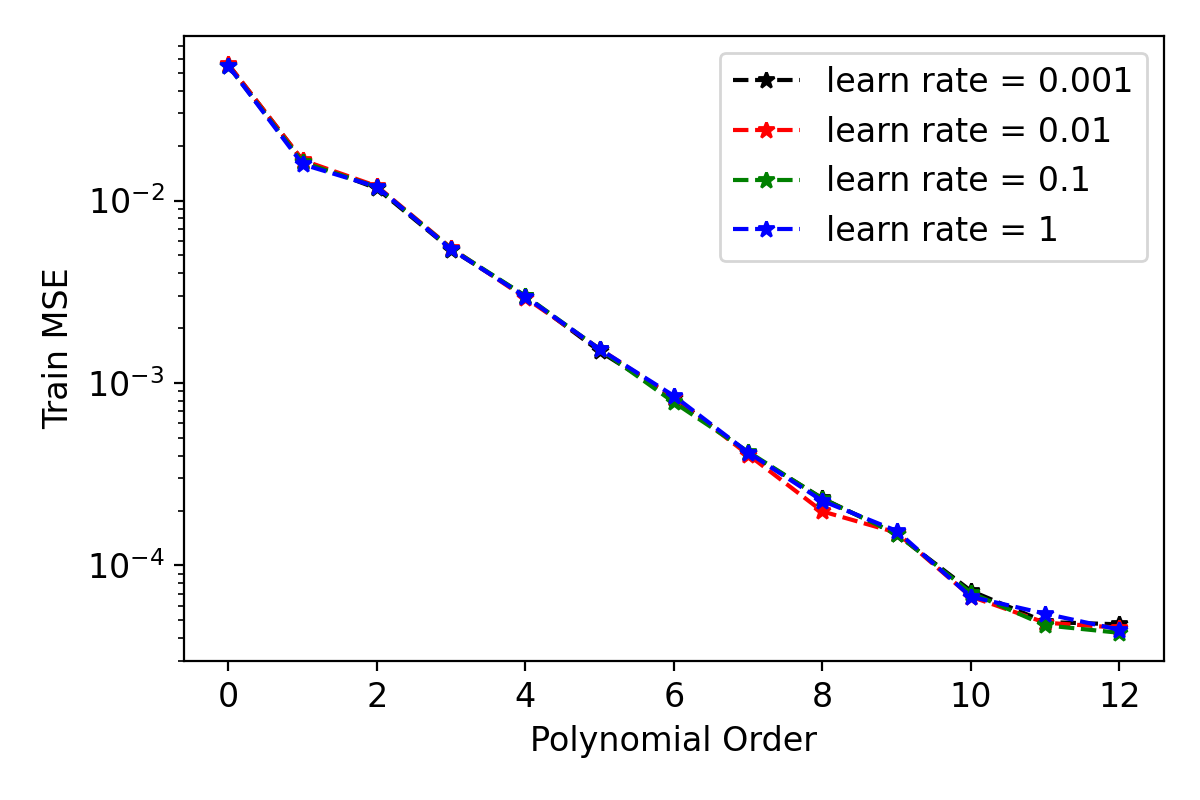
\includegraphics[width=.9\linewidth]{Images/olssgd2.png}
  \caption{}
  \label{fig:olssgd2}
\end{subfigure}%
\begin{subfigure}{.5\textwidth}
  \centering
  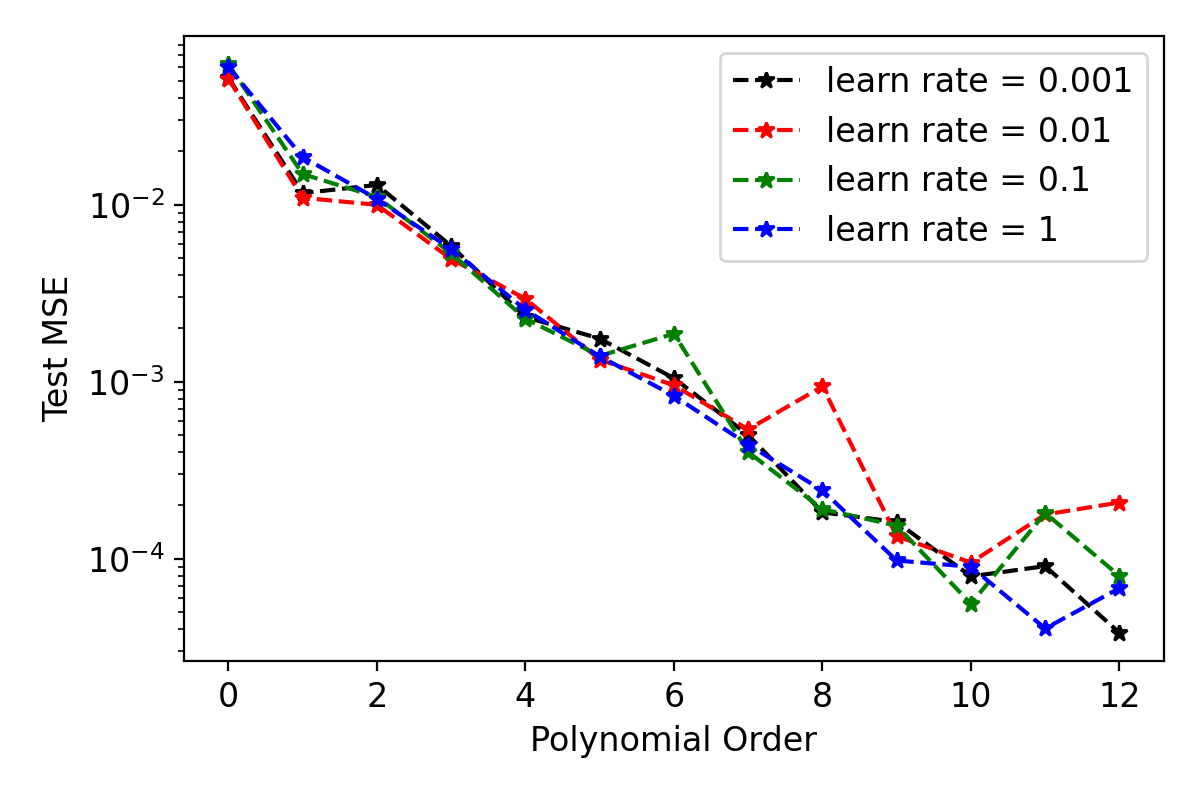
\includegraphics[width=.9\linewidth]{Images/olssgd1.png}
  \caption{}
  \label{fig:olssgd1}
\end{subfigure}
\caption{For $r=0.1$, $var=0$, $n=900$, $num min batches = 32$ and $epochs=10$: (a) $MSE_{train}$ and (b) $MSE_{test}$ plotted as functions of model complexity for varying learn rate}
\label{fig:ols sgd learnrate}
\end{figure}


\begin{figure}
\centering
\begin{subfigure}{.5\textwidth}
  \centering
  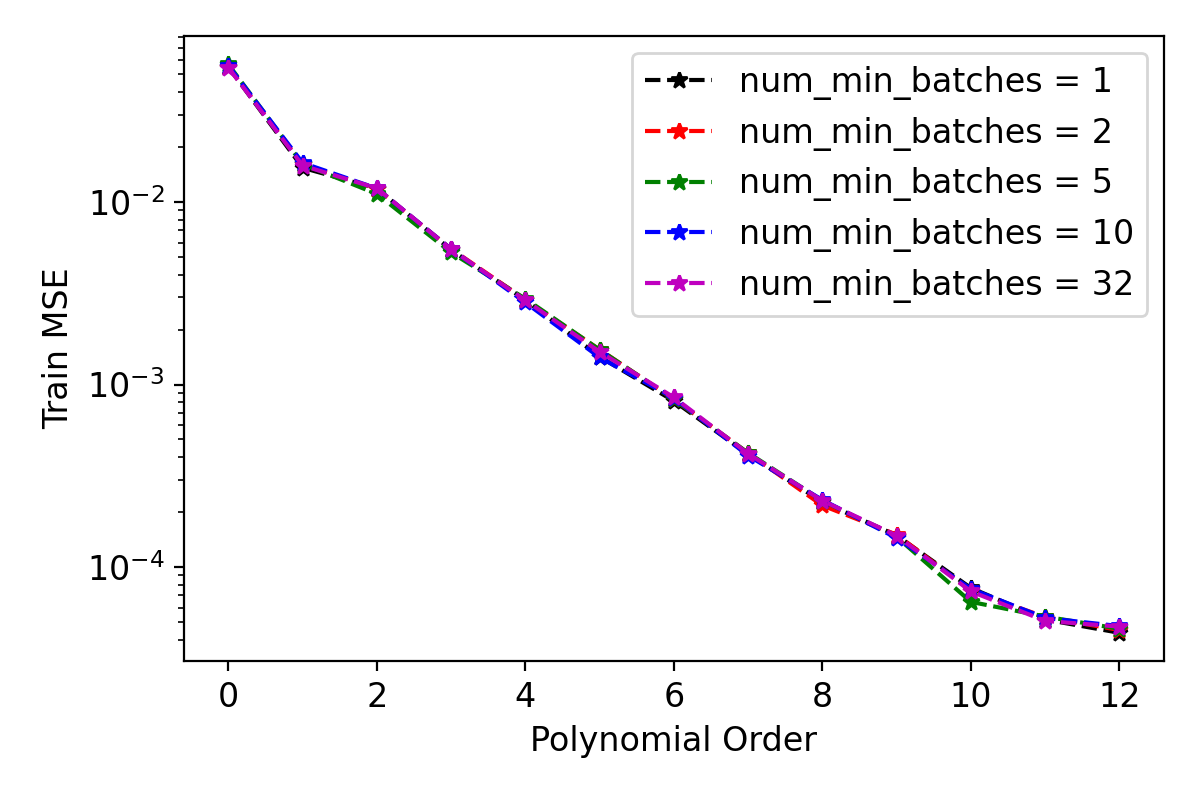
\includegraphics[width=.9\linewidth]{Images/olssgd4.png}
  \caption{}
  \label{fig:olssgd4}
\end{subfigure}%
\begin{subfigure}{.5\textwidth}
  \centering
  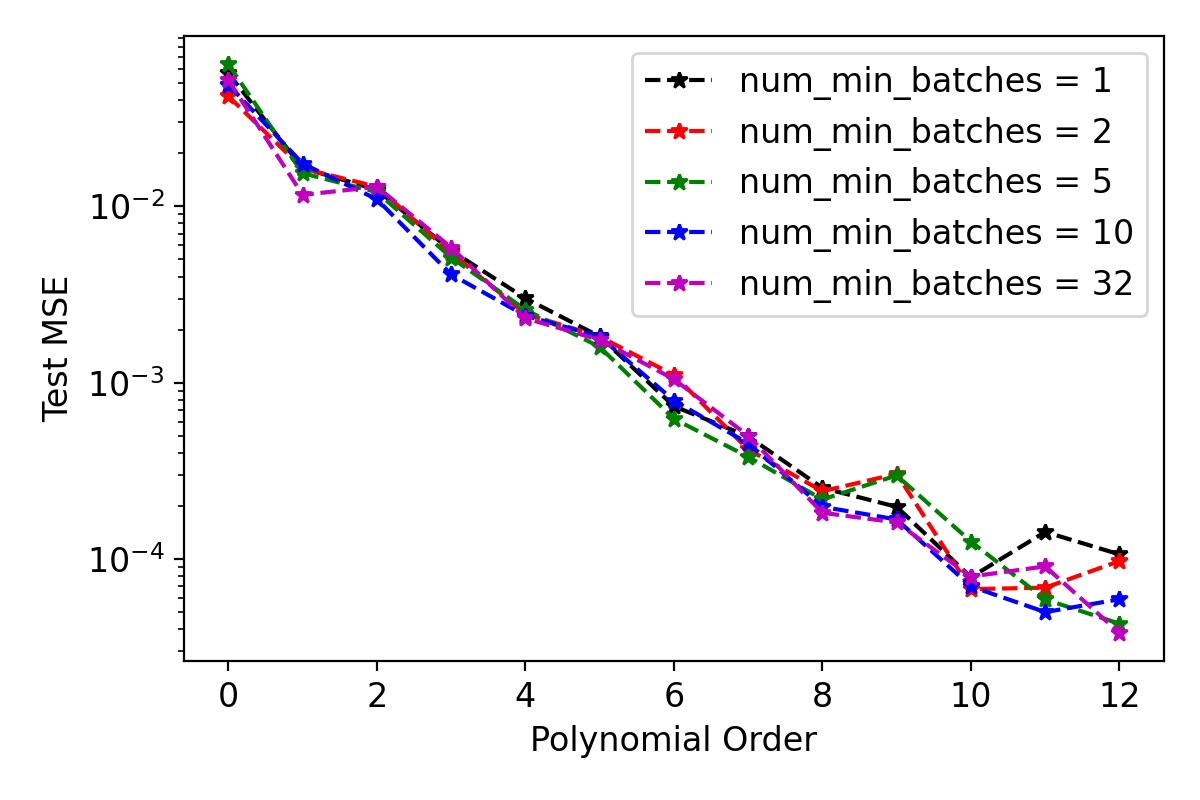
\includegraphics[width=.9\linewidth]{Images/olssgd3.png}
  \caption{}
  \label{fig:olssgd3}
\end{subfigure}
\caption{For $r=0.1$, $var=0$, $n=900$, $learn rate = 0.001$ and $epochs=10$: (a) $MSE_{train}$ and (b) $MSE_{test}$ plotted as functions of model complexity for varying number of min batches}
\label{fig:ols sgd num min batches}
\end{figure}

\begin{figure}
\centering
\begin{subfigure}{.5\textwidth}
  \centering
  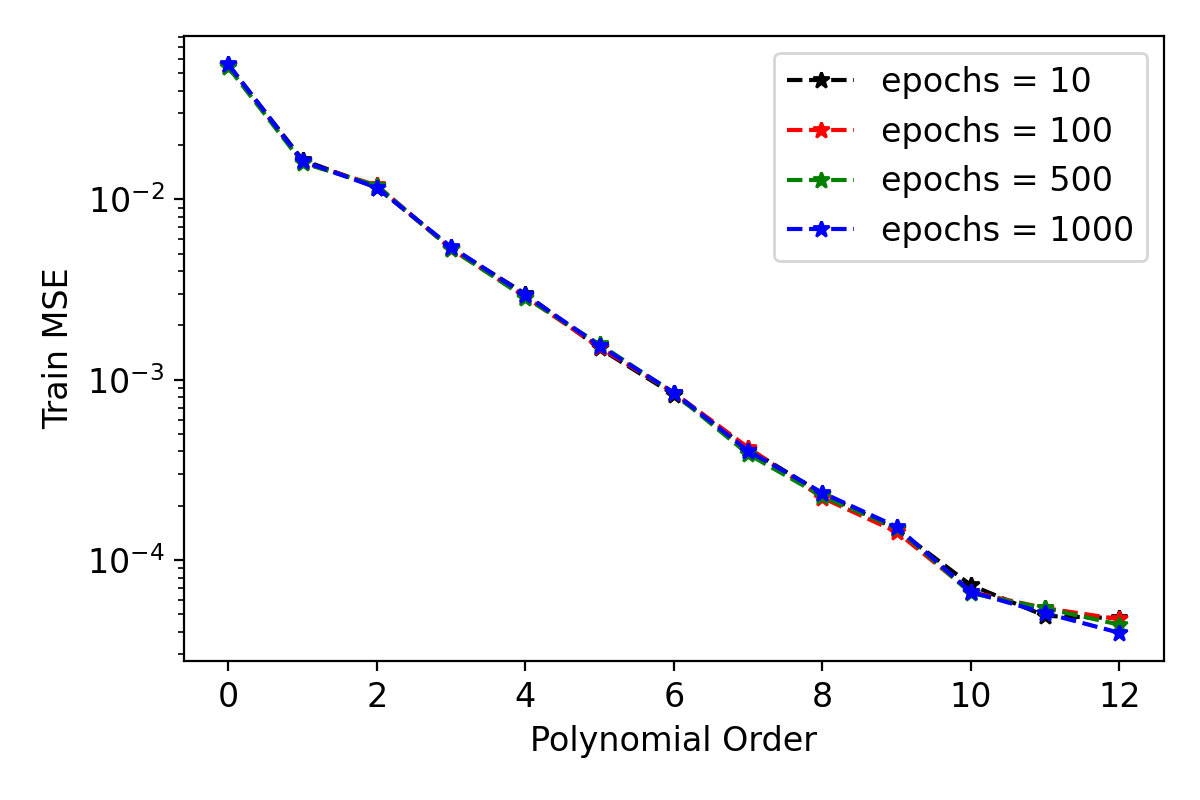
\includegraphics[width=.9\linewidth]{Images/olssgd6.png}
  \caption{}
  \label{fig:olssgd6}
\end{subfigure}%
\begin{subfigure}{.5\textwidth}
  \centering
  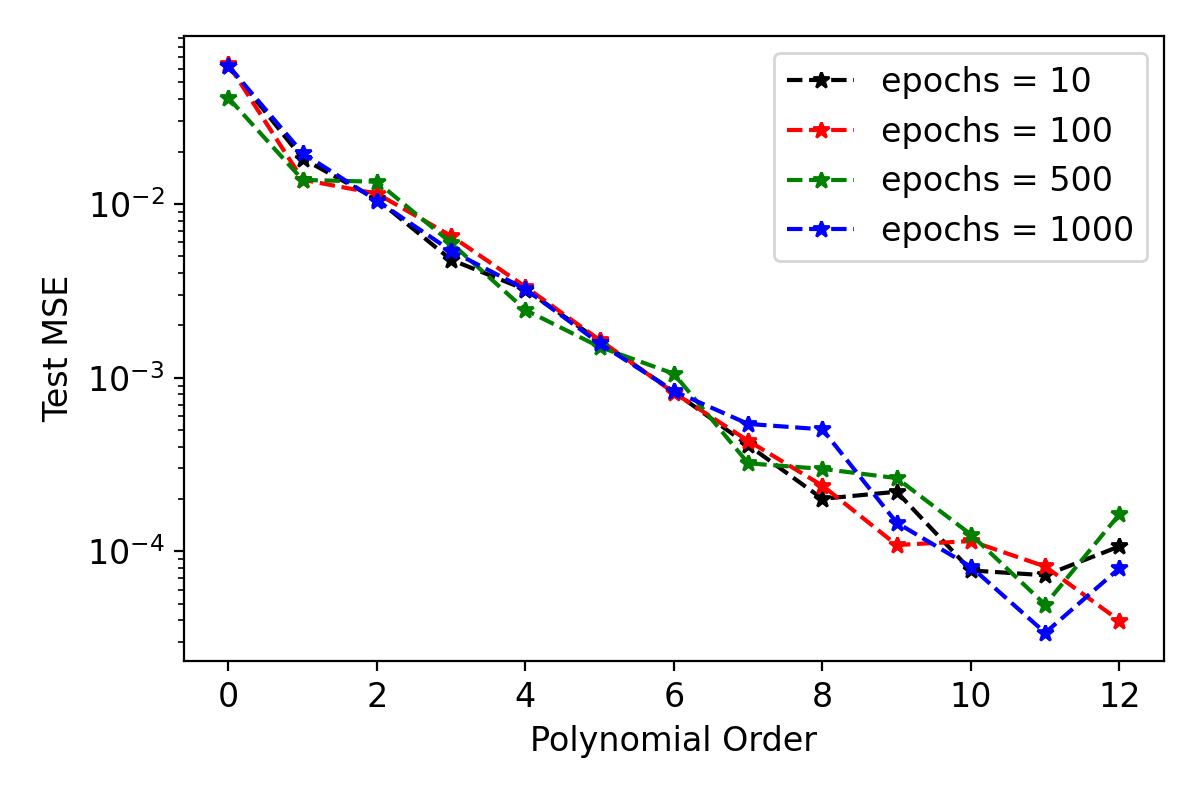
\includegraphics[width=.9\linewidth]{Images/olssgd5.png}
  \caption{}
  \label{fig:olssgd5}
\end{subfigure}
\caption{For $r=0.1$, $var=0$, $n=900$, $learn rate = 0.001$ and $num min batches=32$: (a) $MSE_{train}$ and (b) $MSE_{test}$ plotted as functions of model complexity for varying number of epochs}
\label{fig:ols sgd epochs}
\end{figure}